\documentclass[10pt,letterpaper,journal]{IEEEtran}
\usepackage[letterpaper,margin=1in]{geometry}
\usepackage{amsmath,amsfonts}
\usepackage{algorithmic}
\usepackage{algorithm}
\usepackage{array}
\usepackage{textcomp}
\usepackage{stfloats}
\usepackage{url}
\usepackage{verbatim}
\usepackage{graphicx}
\usepackage{cite}
\usepackage{hyperref}
\usepackage{cleveref}
\usepackage{amssymb}
\usepackage{dsfont}
\newcommand{\mathbbm}[1]{\mathds{#1}}
\usepackage{subcaption}
\usepackage{xcolor}
\newcommand{\revnew}[1]{\textcolor{red}{#1}}
\usepackage{tabularx}
\usepackage{threeparttable}
\usepackage{booktabs}
\usepackage{makecell}
\usepackage{multirow}
\captionsetup[figure]{name=Fig., labelsep=period}
\hyphenation{op-tical net-works semi-conduc-tor IEEE-Xplore}
\renewcommand{\algorithmicrequire}{ \textbf{Input:}}     
\renewcommand{\algorithmicensure}{ \textbf{Output:}}   
\newtheorem{theorem}{Theorem}          
\newtheorem{lemma}{Lemma}             
\newtheorem{proposition}{Proposition}  
\newtheorem{corollary}{Corollary}[theorem] 
\usepackage{needspace}
\begin{document}
\bstctlcite{IEEEcontrol}

\title{Cox-PhysiCK: Physics-Conditioned Temporal Graph Learning for Risk-Aware Handover in Ultra-Dense LEO-NTNs}

\author{Haochen~Liu,
        Ting~Liu,
        Jia~Bi,~\IEEEmembership{Senior Member,~IEEE},
Samuel~Pinilla,~\IEEEmembership{Member,~IEEE},
        Bohan~Li,~\IEEEmembership{Member,~IEEE},
        Luping~Xiang,~\IEEEmembership{Senior Member,~IEEE},
        Jian~Xie,~\IEEEmembership{Member,~IEEE},
        Mingliang~Tao,~\IEEEmembership{Senior Member,~IEEE},
        Ling~Wang
        
\thanks{This work was supported in part by the National Natural Science Foundation of China under Grant No. 62501479, and in part by the Key Research and Development Program of Shaanxi under Grant No. 2025CG-GJHX-20. (Corresponding author: Jia Bi)}
\thanks{H. Liu, T. Liu, J. Xie, M. Tao and L. Wang are with the School of Electronics and Information, Northwestern Polytechnical University, Xi'an 710019, China (email:\{haochenliu, xiejian, mltao, lingwang\}@nwpu.edu.cn; liutingLT@mail.nwpu.edu.cn.)}
\thanks{J. Bi and S. Pinilla are with the Scientific Computing Department, STFC, Rutherford Appleton Laboratory, Didcot OX11 0QX, United Kingdom. (e-mail: Jia.Bi@stfc.ac.uk; samuel.pinilla@correo.uis.edu.co).}
\thanks{B. Li is with the Faculty of Information Science and Engineering, Ocean University of China, Qingdao 266100, China (E-mail: bohan.li@ouc.edu.cn).}
\thanks{L. Xiang is with State Key Laboratory of Novel Software Technology, Nanjing University, Nanjing 210008, China, and School of Intelligent Software and Engineering, Nanjing University (Suzhou Campus), Suzhou (E-mail: luping.xiang@nju.edu.cn).}}


\maketitle
\begin{abstract}
\revnew{Ultra-dense low-Earth-orbit (LEO) non-terrestrial networks (NTNs) exhibit rapid topology evolution and shared satellite-capacity constraints, making handover (HO) a sequential and risk-sensitive control problem. We propose Cox-PhysiCK, a grey-box HO framework combining a Cox-process feasibility prior with physics-conditioned temporal graph learning. Under locally frozen orbital planes and feasibility retention, the prior yields a mean feasible-entry rate and the probability of no new feasible satellite entry over a look-ahead window. These descriptors condition a kernel bank that models residual multi-user interactions, with bounded message amplitudes under the stated kernel assumptions. Controller evaluations use SGP4-propagated synthetic Walker constellations and a shared physical-link environment. Cox-PhysiCK maintains lower outage and conditional HO-failure levels than the two TGN baselines at the reported settings. At 500 users and 2000 satellites over 200 decision epochs, its unconditional outage probability is $3.051\%$, compared with $4.147\%$ for load-aware greedy, and its mean cost per user--epoch is lower by $0.0356$ with outage weight five. These gains coexist with more frequent switching and higher ping-pong probabilities than load-aware greedy, identifying a weight-dependent trade-off between reliability, switching, and load.}
\end{abstract}

\begin{IEEEkeywords}
LEO-NTN, ultra-dense satellite constellations, mobility management, temporal graph networks, \textcolor{blue}{physics-conditioned} machine learning
\end{IEEEkeywords}

\section{Introduction}
\IEEEPARstart{L}{ow} Earth orbit (LEO) satellites complement terrestrial broadband access within the 3GPP non-terrestrial network (NTN) framework~\cite{3gpp_tr38811,3gpp_tr38821,lin2021_5gfromspace}.
\revnew{Their moving footprints and rapidly changing visibility make handover (HO) a recurring requirement for service continuity~\cite{rinaldi2020_ntn_survey}. A currently favorable satellite or beam may soon lose visibility or available resources~\cite{11112684}. In dense constellations, simultaneous user associations further change satellite loads and admission outcomes, creating congestion and repeated switching~\cite{juan2022_handover,aljeri2022_mobility}. A controller therefore needs both a description of future candidate availability and a way to account for the effects of concurrent decisions.}

\subsection{Related Work}
\label{RelatedWork}
\revnew{LEO/NTN handover studies combine link-based rules, analytical models, prediction, and learning~\cite{10443403}. User-centric schemes use buffering and lightweight attachment rules~\cite{9134390}, while QoE-oriented methods incorporate predicted service time and radio resources~\cite{9112229}. Matching and cooperative handover coordinate user satisfaction, power, and switching costs~\cite{10884973,10750324}; conditional and group handover address measurement variation and simultaneous signaling demands~\cite{9771987,10622669,10946034}. These designs motivate considering both temporal service opportunities and shared resource constraints.}

\IEEEpubidadjcol
\revnew{Stochastic geometry provides tractable coverage and interference characterizations through Poisson point processes~\cite{okati2020_downlink,talgat2021_sg}, nonhomogeneous and orbital Cox models~\cite{9681887,choi2024_cox}, and reliability meta-distributions~\cite{10107750}. Heterogeneous-LEO analyses further connect density, altitude, and association to coverage and spectral efficiency~\cite{10533435}. Such open-loop characterizations~\cite{9566290} provide useful priors but do not directly specify how a controller should act when associations change subsequent resource availability. Forecast-based and mobility-aware methods incorporate temporal evolution~\cite{li2020_forecast,hu2018_velocityaware}; continuity, dynamic-networking, and routing-cost formulations connect it to higher-layer objectives~\cite{wang2023_seamless,10002869,cheng2025_routingcost}. Resource-orchestration approaches also coordinate handover, slicing, beam management, and spectrum sharing~\cite{10738455,10795206}.}

\revnew{Learning-based control addresses model mismatch and nonstationary network states~\cite{10409745}. Existing approaches include user-driven access control~\cite{9273081}, DQN handover with feeder/user-link coexistence~\cite{11131136}, graph-based load balancing~\cite{LEE2025239}, protocol learning~\cite{lee2024_protocollearning}, and distributed or hierarchical coordination~\cite{10478861,10751771}. Long-term association costs and load coupling are also studied~\cite{9789983,9210807}, while multi-agent DRL addresses decentralized decisions in changing LEO environments~\cite{10552913,10551688}. The gap addressed here is the integration of explicit candidate-entry priors with learned multi-user effects in temporal graph control under concurrent association.}

\subsection{Contributions}
\revnew{We propose Cox-PhysiCK, which combines a Cox-process candidate-entry prior with physics-conditioned temporal graph learning.}
\textcolor{blue}{SGP4 propagation of the synthetic Walker constellation provides the satellite geometry used to determine visibility and remaining service time.}
\revnew{Known ephemerides make future geometric visibility predictable, but a geometric entry does not guarantee admission after other users request service. We therefore represent entry opportunities separately from realized execution outcomes and learn how shared loads affect candidate scores over successive decisions.}
\revnew{The orbital Cox construction retains dependence induced by shared orbital planes. Under the local approximation, its descriptors are closed-form functions of $\rho$, $\beta$, the current feasibility-retention estimate, and a look-ahead window. They avoid enumerating future entry events, while ephemerides still determine current visibility and candidate residual service time (RST). The factor $\kappa$ calibrates entry intensity. An ephemeris-based alternative uses the same feasibility-retention estimate, isolating the choice of arrival representation. Their relative performance varies with constellation size. The main contributions are:}
\begin{itemize}
    \item \revnew{We formulate causal multi-user HO with endogenous feasibility and derive a Cox descriptor for the probability of no new feasible satellite entry over the residual service interval. Geometry-level arrivals are thinned by SINR and load feasibility under the adopted local approximation. The descriptor summarizes future candidate scarcity for subsequent control decisions.}
    \item \revnew{Cox-PhysiCK embeds feasible-arrival rate, zero-arrival probability, and RST into edge descriptors and }
    \textcolor{blue}{physics-conditioned message kernels}\revnew{. A learned coefficient head mixes these kernels with load and link information to correct analytic candidate utility. Convex mixing bounds message amplitudes under the stated kernel assumptions; the descriptor-to-decision analysis gives a sufficient local margin for preserving a request.}
    \item \revnew{Closed-loop evaluation uses SGP4-propagated synthetic Walker constellations and a shared physical-link and execution interface. Comparisons include rule-based controllers, temporal graph baselines, and LEO-MADRL over up to 800 epochs and 500 users. The results identify reliability--switching trade-offs and lower mean cost than load-aware greedy at high user density. Parameter-matched message variants and separate descriptor interventions examine the kernel bank and arrival representation, while calibration, cost-weight, and hysteresis studies characterize sensitivity.}
\end{itemize}

\revnew{\textit{Notation}: Scalars, vectors, and sets use italic, bold lowercase, and calligraphic symbols. $\mathbb E[\cdot]$, $|\cdot|$, $\|\cdot\|$, $(\cdot)^\top$, and $\mathbf1\{\cdot\}$ denote expectation, cardinality, Euclidean norm, transpose, and indicator; $[\mathbf x\Vert\mathbf y]$ denotes concatenation.}


\begin{figure}[!t]
    \centering
    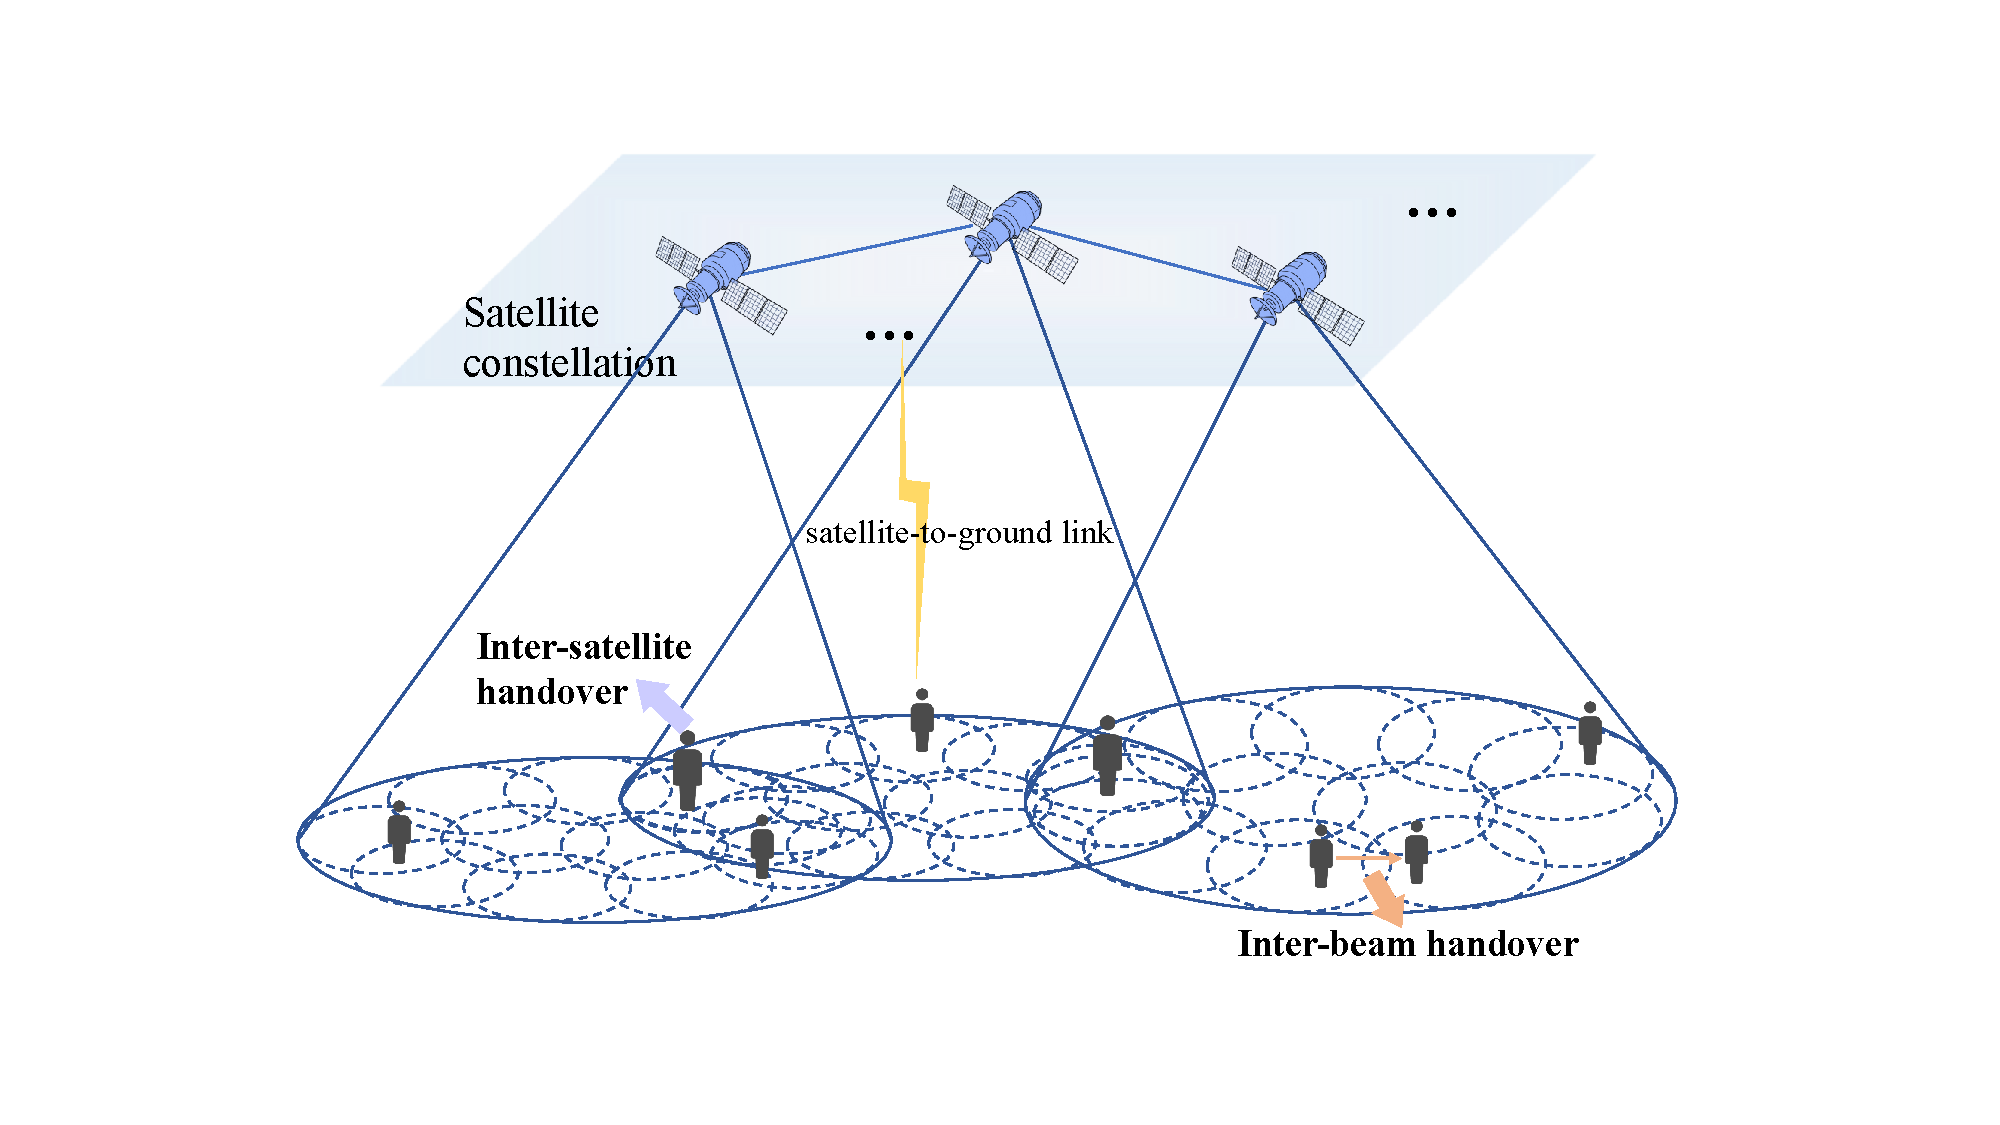
\includegraphics[width=0.9\linewidth,trim =120pt 75pt 120pt 90pt, clip ]{figures/figure_1.pdf}
    \caption{Illustration of a LEO satellite network with multiple orbital planes and multi-beam satellites. The network supports inter-beam and inter-satellite handovers.}
    \label{fig:system_model}
\end{figure}


\section{System Model and Problem Formulation}
\label{systemmodel}
\revnew{The downlink in Fig.~\ref{fig:system_model} serves $K$ terrestrial UEs indexed by $\mathcal{K}=\{1,\ldots,K\}$. Each satellite generates up to $N$ reconfigurable spot beams. At epochs $t\in\{0,\Delta t,2\Delta t,\ldots\}$, satellites enable beam subsets, and each UE associates with at most one satellite-beam pair.}

\vspace{-2mm}
\subsection{Orbital and Constellation Model}
\label{subsec:orbit}

\revnew{The orbital shell has radius $R\!=\!R_e\!+\!h$, with Earth radius $R_e$ and altitude $h$.}
\textcolor{blue}{To retain the dependence induced by shared orbital planes, we use a Cox approximation of the constellation.}
\revnew{Orbital planes form a PPP on $(\Omega,\varphi)\in[0,2\pi)\times[0,\pi]$ with intensity}
\begin{equation}
 \lambda_{\rm pl}(\Omega,\varphi)
 =
 \frac{P}{2\pi}\frac{\sin\varphi}{2},
 \label{eq:lambda_pl}
\end{equation}
\revnew{Here, $\Omega$ is the right ascension of the ascending node, $\varphi$ is orbital inclination, and $P$ is the mean plane count.}

\revnew{Conditioned on each plane, satellite phases form independent one-dimensional PPPs on $\omega\in[0,2\pi)$ with intensity}
\begin{equation}
 \lambda_{\rm sat}(\omega)
 =
 \frac{Q}{2\pi}.
 \label{eq:lambda_sat}
\end{equation}
\revnew{Here, $\omega$ is orbital phase and $Q$ the mean satellites per plane.}
\revnew{The expected size is $O=PQ$. In a realized satellite set $\mathcal S_{\rm sat}$, $\nu\in\mathcal S_{\rm sat}$ indexes a satellite and $(\nu,n)$ its $n$-th beam.}

\revnew{Elevation $\varepsilon_{k,\nu}(t)$ and minimum mask $\varepsilon_{\min}$ define UE $k$'s visible satellites:}
\begin{equation}
\mathcal C_k(t)
\triangleq
\left\{
\nu\in\mathcal S_{\rm sat}:
\varepsilon_{k,\nu}(t)\ge \varepsilon_{\min}
\right\}.
\label{eq:visible_satellite_set}
\end{equation}
\textcolor{blue}{On the spherical shell, this elevation requirement defines a visible cap with Earth-centered half-angle}
\begin{equation}
\textcolor{blue}{
\alpha
=\arccos\!\left(\frac{R_e}{R}\cos\varepsilon_{\min}\right)
-\varepsilon_{\min}.}    
\label{half_angle}
\end{equation}

\revnew{Let $\mathcal N_\nu(t)$ contain satellite $\nu$'s scheduled enabled beams under time-domain beam hopping. UE $k$'s visible satellite-beam candidates are}
\begin{equation}
\mathcal V_k(t)
\triangleq
\left\{
(\nu,n):
\nu\in\mathcal C_k(t),\;
n\in\mathcal N_\nu(t)
\right\}.
\label{eq:visible_beam_candidate_set}
\end{equation}

\revnew{Orbital motion changes $\mathcal C_k(t)$, with new entries during $(t-\Delta t,t]$ counted as}
\begin{equation}
N^{\rm in}_{k}(t)
\triangleq
\left|
\mathcal C_k(t)
\setminus
\mathcal C_k(t-\Delta t)
\right|.
\label{eq:new_visible_satellite_count}
\end{equation}
\revnew{The geometry-level entry rate $\Lambda^{\rm leo}$ gives}
\begin{equation}
\mathbb E\!\left[
N^{\rm in}_{k}(t)
\right]
\approx
\Lambda^{\rm leo}\Delta t .
\label{eq:leo_entry_intensity}
\end{equation}

\textcolor{blue}{The number of orbital planes intersecting the visible cap is Poisson distributed with mean $\rho=PP_{\rm in}$, where $P_{\rm in}=\sin\alpha$.
For the temporal entry prior, their Earth-fixed orientations are locally fixed over a window shorter than one orbital period.
The mean geometry-level entry rate is then given by}
\begin{equation}
\textcolor{blue}{
\Lambda^{\rm leo}
=\rho\beta
=\kappa(PP_{\rm in})\frac{Q\theta}{2\pi}.
}
\label{eq:Lambda_leo_form}
\end{equation}
\revnew{Here, $\theta$ is orbital phase angular speed, and $\beta=\kappa Q\theta/(2\pi)$ scales the ideal per-plane rate $Q\theta/(2\pi)$ by the dimensionless factor $\kappa$.}
\revnew{Under \eqref{eq:lambda_pl}, the projection of a unit plane normal onto the user's radial direction is uniform on $[-1,1]$; cap intersection requires absolute projection at most $\sin\alpha$, giving $P_{\rm in}=\sin\alpha$. This factor enters only through $\rho$. The factor $\kappa$ calibrates the ideal entry intensity for inclined Walker geometry and user latitudes; $p_{{\rm feas},k}(t)$ separately applies feasibility filtering.}


\revnew{For $\nu\in\mathcal C_k(t)$, the geometric remaining visibility time, termed RST, is}
\begin{equation}
T^{\rm rst}_{\nu,k}(t)
\triangleq
\Delta t\cdot
\min
\left\{
m\ge 1:
\nu\notin \mathcal C_k(t+m\Delta t)
\right\}.
\label{eq:geometry_rst}
\end{equation}
\revnew{RST describes geometric visibility; beam availability, capacity, and link quality may change within this interval.}


\vspace{-2mm}
\subsection{Channel and Load Model}
\label{subsec:link}

\textcolor{blue}{
\revnew{We model large-scale propagation without small-scale fading. Each admitted UE occupies a fixed $B$-wide subband during epoch data transmission. Subbands align across beams, and same-beam users receive orthogonal subbands. With fixed power $P_{\rm tx}$ per occupied subband, beam $(\nu,n)$ delivers}
\begin{equation}
P_{k,\nu,n}(t)
=P_{\rm tx}G_{k,\nu,n}(t)G^{\rm rx}_{k,\nu}(t)
L_{k,\nu}(t),
\label{eq:received_power}
\end{equation}
\revnew{where $G_{k,\nu,n}(t)$ is transmit gain from footprint/pointing geometry, $G^{\rm rx}_{k,\nu}(t)$ is UE receive gain, and}
\begin{equation}
L_{k,\nu}(t)
=
\left(\frac{\lambda}{4\pi d_{k,\nu}(t)}\right)^2
10^{-A_{k,\nu}(t)/10},
\label{eq:large_scale_gain}
\end{equation}
\revnew{is the large-scale propagation gain. Here, $\lambda=c/f_c$, with light speed $c$, carrier $f_c$, and satellite--UE range $d_{k,\nu}(t)$. Additional attenuation is}
\begin{equation}
A_{k,\nu}(t)
=A^{\rm gas}_{k,\nu}(t)+A^{\rm rain}_{k,\nu}(t)
+A^{\rm blk}_{k,\nu}(t),
\label{eq:additional_attenuation}
\end{equation}
\revnew{where $A^{\rm gas}_{k,\nu}(t)$, $A^{\rm rain}_{k,\nu}(t)$, and $A^{\rm blk}_{k,\nu}(t)$ represent gas, rain, and blockage losses.} 
}


\textcolor{blue}{
\revnew{Subbands are orthogonal across all beams of a satellite and fully reused across satellites. Only same-subband transmissions interfere, at most one per beam with power $P_{\rm tx}$; intra-satellite interference is absent. Let $a_k(t)$ be UE $k$'s realized association after admission/execution, $s_k(t)=a_k(t-\Delta t)$ its previous association, and $a_k^{\rm req}(t)$ its request. Active pairs after execution are}}
\begin{equation}
\mathcal B_{\rm act}(t)
\triangleq
\{(\mu,m): \exists k\in\mathcal K,\ a_k(t)=(\mu,m)\}.
\end{equation}
\revnew{Let $\mathcal I_{k,\nu,n}(t)\subseteq \mathcal B_{\rm act}(t)\setminus\{(\nu,n)\}$ contain other active beams on UE $k$'s $B$-wide subband. Each $(\mu,m)\in\mathcal I_{k,\nu,n}(t)$ contributes received interference $P_{k,\mu,m}(t)$. All powers in a tagged-link SINR use the same receive orientation, suppressed in the gain notation; interfering gains use angles relative to this orientation.}
The downlink SINR is
\begin{equation}
\gamma_{k,\nu,n}(t)=
\frac{P_{k,\nu,n}(t)}
{\sum\limits_{(\mu,m)\in \mathcal{I}_{k,\nu,n}(t)} P_{k,\mu,m}(t) + \sigma^2},
\label{eq:sinr_sys_rev}
\end{equation}
\textcolor{blue}{where $\sigma^2$ is the noise power over the allocated bandwidth $B$.}
\revnew{The downlink rate is}
\begin{equation}
R_{k,\nu,n}(t) =
B \log_2 \left( 1 + \gamma_{k,\nu,n}(t) \right),
\label{eq:rate_def}
\end{equation}

The load of satellite $\nu$ after all association decisions is
\begin{equation}
\ell_\nu(t)=\sum_{k\in\mathcal{K}}\sum_{n\in\mathcal{N}_\nu(t)}\mathbbm{1}\{a_k(t)=(\nu,n)\},
\label{eq:load_sys_rev}
\end{equation}
where $\ell_\nu^{\max}$ denotes the maximum admissible satellite load.

\revnew{Simultaneous decisions use frozen observations.}
\revnew{The broadcast occupancy is $\tilde{\ell}_\nu(t)=\ell_\nu(t-\Delta t)$. Let $\iota_{k,\nu}(t)$ indicate whether $s_k(t)$ belongs to satellite $\nu$, with $\iota_{k,\nu}(t)=0$ for $s_k(t)=\emptyset$. The candidate load is}
\begin{equation}
\textcolor{blue}{
\tilde{\ell}_{\nu,k}^{+}(t)
=
\tilde{\ell}_\nu(t)+1-\iota_{k,\nu}(t).}    
\end{equation}
\revnew{The pre-execution SINR $\tilde{\gamma}_{k,\nu,n}(t)$ uses current geometry and the preceding epoch's realized co-channel occupancy, with no additional observation noise. Both $\gamma$ and $\tilde\gamma$ are linear power ratios; dB thresholds are converted before comparison. UE $k$'s observable feasible set is}
\begin{equation}
\textcolor{blue}{
\begin{aligned}
\tilde{\mathcal A}_k(t)=\bigl\{(\nu,n)\in\mathcal V_k(t):\;&
\tilde\gamma_{k,\nu,n}(t)\ge\gamma_{\min},\\
&\tilde\ell_{\nu,k}^{+}(t)\le\ell_\nu^{\max}\bigr\}.
\end{aligned}
}
\label{eq:observable_feasible_set}
\end{equation}
Here, $\gamma_{\min}$ denotes the minimum SINR threshold.
\revnew{The fraction of visible satellites with an observably feasible beam is}
\begin{equation}
p_{{\rm feas},k}(t)=
\begin{cases}
\displaystyle
\frac{\sum_{\nu\in\mathcal C_k(t)}
\mathbf 1\!\left\{\substack{\exists n\in\mathcal N_\nu(t):\\
(\nu,n)\in\tilde{\mathcal A}_k(t)}\right\}}
{|\mathcal C_k(t)|},
& |\mathcal C_k(t)|>0,\\[4pt]
0,& |\mathcal C_k(t)|=0.
\end{cases}
\label{eq:p_feas}
\end{equation}
\revnew{The exact visible-satellite count is the denominator; an empty visible set gives zero.}

\revnew{All methods form $\mathcal V_k^{\rm pre}(t)$ from at most $K_c$ pairs in $\mathcal V_k(t)$, ranked by decreasing frozen $\tilde\gamma_{k,\nu,n}(t)$. An excluded feasible serving pair replaces the lowest-ranked pair. An infeasible serving pair is excluded from the decision set}
\begin{equation}
\textcolor{blue}{
\mathcal D_k(t) 
=\mathcal V_k^{\rm pre}(t)\cap\tilde{\mathcal A}_k(t).}  
\end{equation}


\vspace{-2mm}
\subsection{Handover Actions, Costs, and Analytic Utility}
\label{subsec:action_cost}

\textcolor{blue}{\revnew{UE $k$ requests an association from}
\begin{equation}
a_k^{\rm req}(t)\in\mathcal D_k(t)\cup\{\emptyset\},
\label{eq:action_sys_rev}
\end{equation}
\revnew{where $\emptyset$ means no request. Admission/execution determines $a_k(t)$, with $a_k(t)=\emptyset$ denoting outage.}}
\revnew{The executed HO indicator is}
\begin{equation}
\mathbbm{1}_k^{\rm HO}(t)\triangleq
\mathbbm{1}\!\left\{\begin{array}{l}
a_k(t)\neq\emptyset,\ a_k(t-\Delta t)\neq\emptyset,\\
a_k(t)\neq a_k(t-\Delta t)
\end{array}\right\}.
\label{eq:ho_indicator}
\end{equation}
\textcolor{blue}{\revnew{Dimensionless candidate HO overhead is}
\begin{equation}
C_{k,\nu,n}(t)=
\begin{cases}
0,
& s_k(t)=\emptyset \text{ or } s_k(t)=(\nu,n),\\
c_{\rm ib},
& s_k(t)=(\nu,m),\ m\neq n,\\
c_{\rm is},
& s_k(t)=(\mu,m),\ \mu\neq\nu,
\end{cases}    
\end{equation}
\revnew{where $c_{\rm ib}$ and $c_{\rm is}$ are inter-beam and inter-satellite overheads; retention and initial access cost zero. For $a_k(t)=(\nu,n)\neq\emptyset$, set $C_k^{\rm exec}(t)=C_{k,\nu,n}(t)$; for $a_k(t)=\emptyset$, set $C_k^{\rm exec}(t)=0$.}}

\revnew{The instantaneous per-user cost is}
\begin{equation}
\begin{aligned}
c_k(t) &= w_o\mathbbm{1}\{a_k(t)=\varnothing\}
          +w_h C_k^{\rm exec}(t)\\
       &+w_\ell\mathbbm{1}\{a_k(t)\neq\varnothing\}
          \textcolor{blue}{\bar{\ell}_{\nu_k}(t)}\\
       &-w_r\mathbbm{1}\{a_k(t)\neq\varnothing\}
          \textcolor{blue}{\bar{R}_{k,\nu,n}(t)},
\end{aligned}
\label{eq:instantaneous_cost}
\end{equation}
\textcolor{blue}{where the normalized load and rate are defined as}
\begin{equation}
\begin{aligned}
\textcolor{blue}{\bar{\ell}_{\nu_k}(t)}
&\textcolor{blue}{=
\frac{\ell_{\nu_k}(t)}{\ell_{\nu_k}^{\max}},}\quad
\textcolor{blue}{\bar{R}_{k,\nu,n}(t)}
\textcolor{blue}{=
\frac{R_{k,\nu,n}(t)}{R_{\rm ref}}.}
\end{aligned}
\label{eq:normalized_load_rate}
\end{equation}
\revnew{The weights $\{w_o,w_h,w_\ell,w_r\}$ are nonnegative, $\ell_\nu^{\max}$ is satellite capacity, and $R_{\rm ref}>0$ is a fixed reference rate. For $a_k(t)\neq\varnothing$, $(\nu,n)=a_k(t)$ and $\nu_k=\nu$; for $a_k(t)=\varnothing$, both load and rate terms are zero.}

\textcolor{blue}{\revnew{For $(\nu,n)\in\tilde{\mathcal A}_k(t)$, the corresponding analytic utility is}
\begin{equation}
U^{\rm ana}_{k,\nu,n}(t)
=
w_r\bar R^{\rm obs}_{k,\nu,n}(t)
-w_h C_{k,\nu,n}(t)
-w_\ell\overline{\tilde{\ell}}_{\nu,k}^{+}(t),
\label{eq:analytic_utility}
\end{equation}
where
\[
\bar R^{\rm obs}_{k,\nu,n}(t)
=
{R^{\rm obs}_{k,\nu,n}(t)}/{R_{\rm ref}},
\quad
\overline{\tilde{\ell}}_{\nu,k}^{+}(t)
=
{\tilde{\ell}_{\nu,k}^{+}(t)}/{\ell_\nu^{\max}},
\]
\revnew{and $R^{\rm obs}_{k,\nu,n}(t) = B\log_2\!\left(1+\tilde\gamma_{k,\nu,n}(t)\right)$ uses frozen decision-time SINR. With the same weights as the realized cost, $U^{\rm ana}_{k,\nu,n}(t)$ approximates its negative non-outage component using observed rate and candidate load.}}




\vspace{-2mm}
\subsection{Problem Formulation}
\label{subsec:problem}

\revnew{The decision state $\boldsymbol{\xi}(t)$ contains beam configuration, visible candidates, observed SINR, delayed load, and past associations.}
\revnew{A causal policy $\pi$ maps $\{\boldsymbol{\xi}(\tau)\}_{\tau\le t}$ to joint requests $\mathbf a^{\rm req}(t)=\{a_k^{\rm req}(t)\}_{k\in\mathcal K}$. It seeks the minimum long-term expected cost of realized associations:}
\begin{equation}
\begin{aligned}
\mathcal P_0:\quad &
\min_{\pi}\quad
\limsup_{T\to\infty}
\frac{\textcolor{blue}{\Delta t}}{T}
\mathbb E_{\pi}
\left[
\sum_{t=0,\Delta t,\ldots}^{T-\Delta t}
\sum_{k\in\mathcal K}
c_k(t)
\right] \\
\mathrm{s.t.}\quad&
\textcolor{blue}{a_k^{\rm req}(t)\in\mathcal D_k(t)\cup\{\emptyset\},}
\quad \forall k\in\mathcal K,\ \forall t .
\end{aligned}
\label{eq:problem_sys}
\end{equation}
\revnew{The duration $T$ contains $T/\Delta t$ decision epochs; $\Delta t/T$ yields average network cost per epoch. Orbital motion and beam hopping change $\tilde{\mathcal A}_k(t)$, while concurrent associations determine realized SINR and load. We therefore augment the analytic utility \eqref{eq:analytic_utility} with learned residual multi-user coupling.}



\section{Cox-PhysiCK: Physics-Conditioned Risk-Aware Handover Control}
\label{ProposedMethod}

\begin{figure*}[ht]
  \centering
  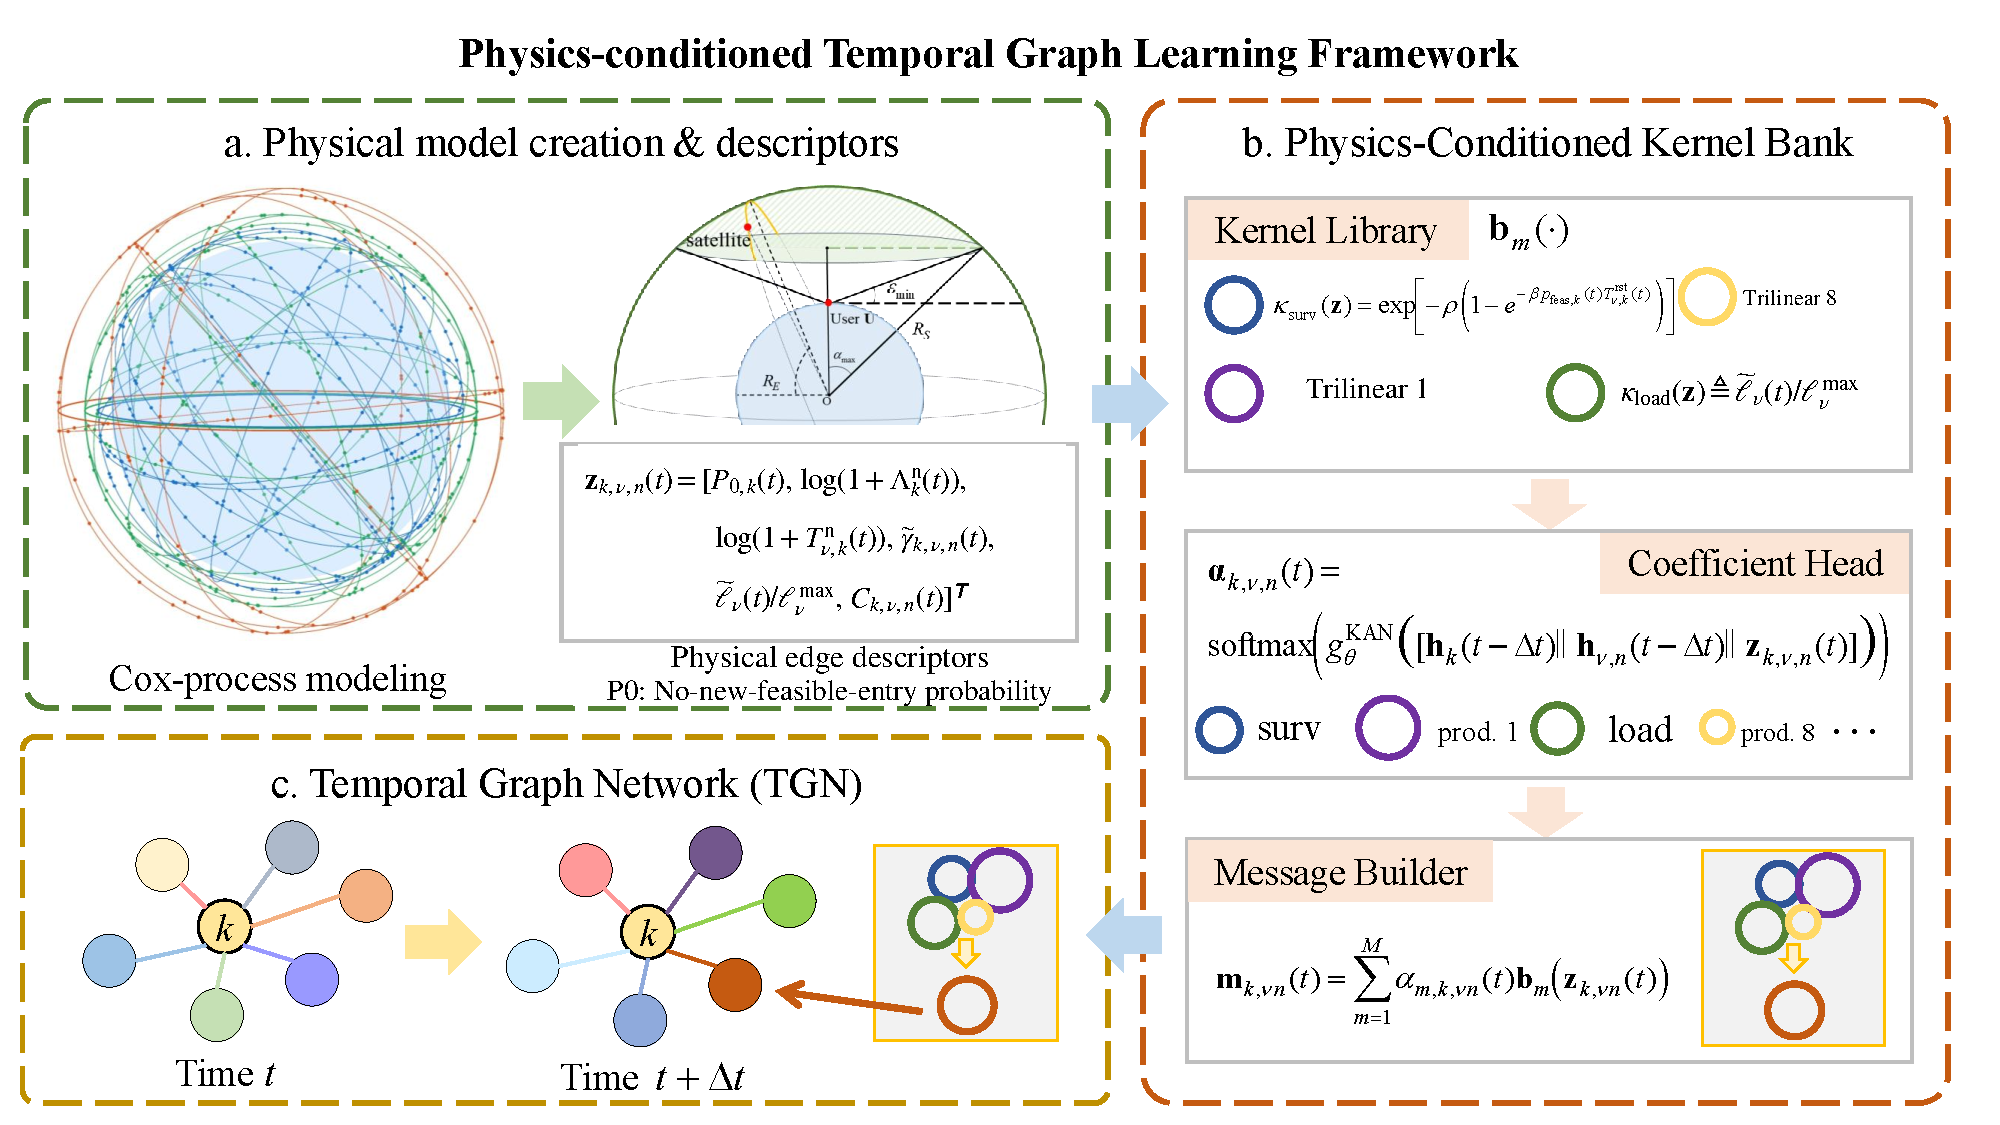
\includegraphics[width=0.95\linewidth]{figures/figure_2.pdf}
  \caption{Overview of the proposed Cox-PhysiCK framework. 
  (a) Cox-process-based constellation modeling and \textcolor{blue}{physical descriptor construction}. 
  (b) Message generation and aggregation via the PhysiCK kernel bank. \revnew{The bank contains eight trilinear product kernels, one zero-arrival kernel, and one load kernel.} 
  (c) Spatio-temporal representation learning using a TGN for multi-user HO control.}
  \label{fig:PhysiCK_TGN}
\end{figure*}


\revnew{Figure~\ref{fig:PhysiCK_TGN} shows Cox-PhysiCK. Cox entry descriptors and geometry-based RST condition a physical kernel bank; a Kolmogorov--Arnold network (KAN)~\cite{liu2025kan} mixes its responses within a temporal graph network (TGN)~\cite{rossi2020temporal}. The resulting residual corrects analytic utility for multi-user interactions.}

\subsection{\textcolor{blue}{Probability of No New Feasible Entry}}
\label{subsec:cox_main}

\textcolor{blue}{For UE $k$, the window $T$ is the remaining service time of its previous serving satellite when that satellite is still visible; otherwise, we set $T=\Delta t$.
This window is shared by all candidate edges of UE $k$.
A feasible arrival is a newly visible satellite with at least one scheduled enabled beam satisfying the observable SINR and load criteria in \eqref{eq:observable_feasible_set}.
Feasibility thinning gives the mean feasible-arrival rate}
\begin{equation}
\Lambda_k^{\rm feas}(t)=\Lambda^{\rm leo}\,p_{{\rm feas},k}(t).
\label{eq:Lambda_feas_main}
\end{equation}
\textcolor{blue}{At each decision epoch $t$, we approximate the future feasibility-retention profile by $\bar p_{k,j|t}=p_{{\rm feas},k}(t)$.
This locally constant profile is recomputed at each decision epoch.}

\textcolor{blue}{Let $M_k(t)\sim\operatorname{Poisson}(\rho)$ be the number of entry-capable planes in the locally frozen-plane model.
Given $M_k(t)$, the entry intensity in interval $j$ is $M_k(t)\beta\bar p_{k,j|t}$.
The mean feasible-entry count per plane over the window is}
\begin{equation}
\textcolor{blue}{
A_k^\Delta(t,T)
=\beta\sum_{j=0}^{J(T)-1}\bar p_{k,j|t}\,\delta_j(T),}    
\end{equation}
\textcolor{blue}{where $J(T)=\lceil T/\Delta t\rceil$ and $\delta_j(T)=\min\{\Delta t,T-j\Delta t\}$.
Denoting the number of feasible arrivals by $N_k^{\rm feas}(t,T)$, the probability of no new feasible entry is}
\begin{equation}
\textcolor{blue}{
\begin{aligned}
P_{0,k}(t)
&\triangleq\Pr\!\left\{N_k^{\rm feas}(t,T)=0\right\}\\
&=\exp\!\left[-\rho\left(1-e^{-A_k^\Delta(t,T)}\right)\right].
\end{aligned}}
\label{eq:Prisk_def_main}
\end{equation}
\textcolor{blue}{Eq.~\eqref{eq:Prisk_def_main} averages the conditional Poisson void probability over orbital planes (Appendix~\ref{app:cox_risk}) to describe new-entry scarcity.}
\revnew{This probability concerns new entries rather than currently available candidates or the outcome of an attempted handover. Admission and execution outcomes enter the conditional HO-failure metric in \eqref{eq:metric_fail}.}



\vspace{-4mm}
\subsection{PhysiCK-TGN Backbone: Temporal Coupling with Physics-Conditioned Kernels}
\label{subsec:physick_main}

At each epoch $t$, we construct a bipartite dynamic graph
$\mathcal{G}(t)=(\mathcal{K}\cup\mathcal{B}(t),\mathcal{E}(t))$.
\revnew{The calligraphic $\mathcal B(t)$ denotes beam nodes, while the scalar $B$ denotes bandwidth.}
\textcolor{blue}{Here $\mathcal B(t)=\bigcup_k\mathcal V_k^{\rm pre}(t)$ contains the preselected beam nodes, with an edge from each preselecting user. HO decisions remain restricted to $\mathcal D_k(t)$.}
Each node $i\in\mathcal{K}\cup\mathcal{B}(t)$ maintains a temporal memory state $\mathbf{h}_i(t)$, which is updated via message passing:
\begin{align}
\bar{\mathbf{m}}_i(t) &=
\mathrm{AGG}\Big(\{\mathbf{m}_{ji}(t): j\in \mathcal{N}_i(t)\}\Big),
\label{eq:agg_main}\\
\mathbf{h}_i(t) &= \mathrm{GRU}\big(\mathbf{h}_i(t-\Delta t),\bar{\mathbf{m}}_i(t)\big),
\label{eq:gru_main}
\end{align}
\revnew{Here $\mathcal N_i(t)$ is the neighbor set. The same edge message, computed from pre-update memories, is mean-aggregated at both endpoints. Separate shared user and beam GRUs update synchronously once per epoch. Isolated nodes retain memory.}

\textcolor{blue}{We define the normalized arrival-rate and RST inputs as
\begin{equation}
\begin{aligned}
\Lambda_k^{\mathrm n}(t)
\triangleq \Lambda_k^{\rm feas}(t)T_{\rm ref}, \quad T_{\nu,k}^{\mathrm n}(t)
\triangleq T_{\nu,k}^{\rm rst}(t)/T_{\rm ref},
\end{aligned}   
\label{eq:normalized}
\end{equation}
where $T_{\rm ref}$ is a fixed reference time.}
For each candidate edge $(k\!\to\!(\nu,n))$, the edge descriptor is defined as
\begin{equation}
\textcolor{blue}{\begin{aligned}
\mathbf z_{k,\nu,n}(t)
=\big[&
P_{0,k}(t),
\log\!\left(1+\Lambda_k^{\rm n}(t)\right),
\log\!\left(1+{T_{\nu,k}^{\rm n}(t)}\right),\\
&\widetilde{\gamma}_{k,\nu,n}(t),
\widetilde{\ell}_{\nu}(t)/\ell_{\nu}^{\max},
 C_{k,\nu,n}(t)
\big]^{\mathsf T}
\in\mathbb R^{d_z},
\end{aligned}}
\label{eq:z_main}
\end{equation}
\revnew{The first two coordinates describe user-level entry scarcity; the others describe candidate service duration, link, load, and switching cost. PhysiCK constructs the message as}
\begin{equation}
\mathbf{m}_{k,\nu,n}(t)=\sum_{m=1}^{M}\alpha_{m,k,\nu,n}(t)\,\mathbf{b}_m(\mathbf{z}_{k,\nu,n}(t))\in\mathbb{R}^{d_{\rm msg}}.
\label{eq:msg_kernel_main}
\end{equation}
\textcolor{blue}{Physical descriptors determine both the message bases and their mixing coefficients.}

\textcolor{blue}{The kernel library includes a candidate-specific zero-arrival kernel}
\begin{equation}
\textcolor{blue}{
\kappa_{\rm surv}(\mathbf z)
=\exp\!\left[-\rho\left(1-e^{-\beta p_{{\rm feas},k}(t)T_{\nu,k}^{\rm rst}(t)}\right)\right],
}
\label{eq:kappa_surv_main}
\end{equation}
\textcolor{blue}{which evaluates the Cox zero-arrival probability over the candidate RST using the local constant profile $\bar p_{k,j|t}=p_{{\rm feas},k}(t)$.}
\revnew{The bank also contains trilinear bases and $\kappa_{\rm load}(\mathbf z)=\tilde\ell_\nu(t)/\ell_\nu^{\max}$. Each scalar kernel is lifted to a vector basis:}
\begin{equation}
\mathbf{b}_m(\mathbf{z})=\kappa_m(\mathbf{z})\,\mathbf{W}_m\,[1,\tilde{\gamma}_{k,\nu,n},\tilde{\ell}_\nu/\ell_\nu^{\max},\textcolor{blue}{{C}_{k,\nu,n}}]^{\!\top}\!,
\label{eq:b_m_main}
\end{equation}
where $\mathbf{W}_m\!\in\!\mathbb{R}^{d_{\rm msg}\!\times\!4}$.

The separable trilinear kernels are
\begin{equation}
\begin{aligned}
\kappa_{(r,q,u)}(\mathbf z)
={}&\textcolor{blue}{\psi_r(P_{0,k})\psi_q(\log(1+\Lambda_k^{\mathrm n}))}\\
&\textcolor{blue}{\times\psi_u(\log(1+T_{\nu,k}^{\mathrm n})),}
\end{aligned}  
\end{equation}
\revnew{With $n_P=n_\Lambda=n_T=2$ bases per axis, the bank has $M=2^3+2=10$ kernels. The functions $\psi$ include the axis scaling in Appendix~\ref{app:implementation}, which also distinguishes physical bases from internal KAN splines.}

The mixing coefficients are generated by a KAN-based coefficient head:
\begin{equation}
\begin{aligned}
\boldsymbol\alpha_{k,\nu,n}(t)=\mathrm{softmax}\Bigl(g^{\rm KAN}_\theta\bigl(
[&\mathbf{h}_k(t^-)\\
\Vert\mathbf{h}_{(\nu,n)}(t^-)&\Vert\mathbf{z}_{k,\nu,n}(t)]\bigr)\Bigr),
\end{aligned}   
\label{eq:alpha_main}
\end{equation}
\revnew{Here $t^-$ denotes pre-update memory, and softmax enforces simplex mixing. Updated memories produce the residual correction to \eqref{eq:analytic_utility}:}
\begin{equation}
\widehat Q_{k,\nu,n}(t)
=
{\rm MLP}_{\rm out}
\left(
[
\mathbf h_k(t)
\Vert
\mathbf h_{\nu,n}(t)
\Vert
\mathbf z_{k,\nu,n}(t)
]
\right),
\label{eq:residual_score}
\end{equation}
\revnew{The head fits the one-step executed-utility residual $-c_k-U^{\rm ana}_{k,b}$, not a discounted return. Models are selected by finite-horizon validation cost and evaluated against \eqref{eq:problem_sys}; Appendix~\ref{app:training_implementation} specifies the loss.}
The final candidate score is given by
\begin{equation}
\widetilde{U}_{k,\nu,n}(t)
=
U^{\rm ana}_{k,\nu,n}(t)
+
\lambda_Q \widehat Q_{k,\nu,n}(t),
\label{eq:U_final_main}
\end{equation}
where $\lambda_Q$ controls the strength of the learned residual correction.


\textcolor{blue}{At each epoch, UE $k$ evaluates the hybrid utility over $\mathcal D_k(t)$ using the frozen observations.
For a nonempty decision set, let}
\begin{equation}
\textcolor{blue}{
b_k^\star(t)
=
\arg\max_{b\in\mathcal D_k(t)}
\widetilde U_{k,b}(t).}
\label{eq:target_ranking}
\end{equation}
\textcolor{blue}{Ties favor the serving pair, followed by satellite and beam indices.
The requested association is}
\begin{equation}
\textcolor{blue}{
a_k^{\rm req}(t)=
\begin{cases}
\emptyset,
& \mathcal D_k(t)=\emptyset,\\
b_k^\star(t),
& s_k(t)\notin\mathcal D_k(t),\
  \mathcal D_k(t)\ne\emptyset,\\
b_k^\star(t),
& s_k(t)\in\mathcal D_k(t),\
  \Delta U_k(t)>\tau_{\rm hyst},\\
s_k(t),
& \text{otherwise},
\end{cases}
}
\label{eq:ho_selection_rule}
\end{equation}
\textcolor{blue}{where $\Delta U_k(t)= \widetilde U_{k,b_k^\star(t)}(t) -\widetilde U_{k,s_k(t)}(t)$ is evaluated when the serving pair remains feasible.
The nonnegative margin $\tau_{\rm hyst}$ is measured in utility units.
An unavailable serving pair bypasses this comparison.}
\revnew{Cox descriptors enter the edge features and physical kernels, shaping the residual in \eqref{eq:residual_score}. They therefore affect both target ranking in \eqref{eq:target_ranking} and the utility difference $\Delta U_k(t)$ used in \eqref{eq:ho_selection_rule} to request a handover.}



\subsection{\textcolor{blue}{HO Procedure and State Update}}
\label{subsec:ho_procedure}

\textcolor{blue}{
A closed-loop rollout comprises $H$ decision steps at $t_h=t_0+h\Delta t$ and lasts $H\Delta t$.
}

\textcolor{blue}{
At each decision epoch, the following four steps are performed.
All controllers use the same admission and execution rules.
}

\textcolor{blue}{
\textit{Step 1: Observation update and request selection.}
Orbital propagation and the current scheduled beam configuration update visibility and link observations.
These observations and the delayed load broadcasts are used to construct $\mathcal D_k(t_h)$ and update the graph features and model states.
Each UE evaluates the hybrid scores in \eqref{eq:U_final_main} and selects $a_k^{\rm req}(t_h)$ using \eqref{eq:ho_selection_rule}.
}

\textcolor{blue}{
\textit{Step 2: Capacity admission.}
Each satellite reserves source slots for UEs with $s_k(t_h)\in\mathcal D_k(t_h)$ throughout the current epoch.
Same-satellite beam changes use these existing slots. 
New users are admitted within the residual capacity in decreasing order of target link-quality estimates, with ties resolved by UE index.
A rejected request retains its reserved source connection when available; otherwise, the UE enters outage.
}

\textcolor{blue}{
\textit{Step 3: HO execution.}
Existing valid subband assignments are retained; newly admitted users obtain available subbands in admission order. The admitted targets and retained source links are checked simultaneously for visibility and an SINR of at least $\gamma_{\min}$ under this tentative joint resource configuration.
A feasible link becomes $a_k(t_h)$ and retains its subband for the epoch; otherwise, its transmission is removed and $a_k(t_h)=\emptyset$.
}

\textcolor{blue}{
\textit{Step 4: State update.}
After failed transmissions are removed, executed associations determine transmitting beams, subbands, loads, and rates via \eqref{eq:rate_def}. Rates use this final interference configuration, which can differ from the Step~3 check. The next epoch broadcasts $\tilde\ell_\nu(t_{h+1})=\ell_\nu(t_h)$ and returns to Step~1.
}

\revnew{Each epoch reconstructs candidates and recomputes actions from propagated geometry and the preceding joint execution. $H$ counts these updates, whereas $T$ is the descriptor look-ahead window.}

\vspace{-4mm}
\begingroup\color{red}
\subsection{Descriptor-to-Decision Robustness}
\label{subsec:risk_decision_robustness}
The following results characterize descriptor, message, and request sensitivity under the stated local assumptions.

\begin{lemma}[Cox probability error]
\label{lem:cox_risk_calibration}
For fixed $\rho>0$, define
\begin{equation}
\mathcal H_k(t,T)=\int_t^{t+T}\bar\Lambda_k^{\rm feas}(u;t)\,du,
\qquad \bar\Lambda_k^{\rm feas}=\rho\beta\bar p_k.
\label{eq:true_integrated_hazard}
\end{equation}
Let $P_{0,k}=f_\rho(\mathcal H_k)$ and $\widehat P_{0,k}=f_\rho(\widehat{\mathcal H}_k)$, where $f_\rho(x)=\exp[-\rho(1-e^{-x/\rho})]$. For nonnegative integrated rates with $|\widehat{\mathcal H}_k-\mathcal H_k|\le\varepsilon_{\mathcal H}$,
\begin{align}
e^{-\varepsilon_{\mathcal H}}\widehat P_{0,k}
&\le P_{0,k}\le e^{\varepsilon_{\mathcal H}}\widehat P_{0,k},
\label{eq:risk_multiplicative_envelope}\\
|\widehat P_{0,k}-P_{0,k}|
&\le1-e^{-\varepsilon_{\mathcal H}}\le\varepsilon_{\mathcal H}.
\label{eq:risk_additive_error}
\end{align}
\end{lemma}
\begin{IEEEproof}
The exponent map $g_\rho(x)=\rho(1-e^{-x/\rho})$ has derivative in $[0,1]$, giving the multiplicative bound. The additive bound follows from $|e^{-a}-e^{-b}|\le1-e^{-|a-b|}$ for $a,b\ge0$.
\end{IEEEproof}

\begin{theorem}[Decision-margin preservation]
\label{thm:decision_margin_preservation}
Compare scores $S$ and $\widehat S$ on the same decision set, serving association, hysteresis threshold, and tie-breaking rule. For reference top candidates $b_1,b_2$, define
\begin{align}
\Gamma_k&=S_{k,b_1}-S_{k,b_2},\label{eq:score_margin}\\
\epsilon_k&=\max_{b\in\mathcal D_k}|\widehat S_{k,b}-S_{k,b}|.
\label{eq:score_perturbation}
\end{align}
Set $\Gamma_k=+\infty$ for at most one candidate and $\epsilon_k=0$ for an empty set. Both requests coincide whenever
\begin{equation}
\Gamma_k>2\epsilon_k+\tau_{\rm hyst}.
\label{eq:decision_margin_preservation}
\end{equation}
\end{theorem}
\begin{IEEEproof}
Every competing candidate satisfies $\widehat S_{k,b_1}-\widehat S_{k,b}\ge\Gamma_k-2\epsilon_k>\tau_{\rm hyst}$. Thus both score vectors retain $b_1$ if it serves the user, or request it otherwise; empty and singleton sets give identical requests directly.
\end{IEEEproof}

\begin{corollary}[Paired request disagreements]
\label{cor:finite_horizon_flip}
At $t_h=t_0+h\Delta t$, averaging the theorem's pointwise implication gives
\begin{equation}
\begin{aligned}
{\rm DFR}_H&=\frac1{KH}\sum_{k,h}\mathbf1\{\widehat a_k^{\rm req}(t_h)\ne a_k^{\rm req}(t_h)\}\\
&\le\frac1{KH}\sum_{k,h}\mathbf1\{\Gamma_k(t_h)\le2\epsilon_k(t_h)+\tau_{\rm hyst}\}.
\end{aligned}
\label{eq:dfr_bound}
\end{equation}
\end{corollary}

\begin{theorem}[Message bounds]
\label{thm:msg_lipschitz}
Using Euclidean norms unless indicated, for the coefficient-head input $\boldsymbol\xi$ assume $\|\mathbf b_m\|\le B_m$, each basis is $L_m$-Lipschitz, and the logit map is $L_g$-Lipschitz. Let $B_\kappa=\max_mB_m$, $L_\kappa=\max_mL_m$, and use primes for perturbed inputs. Then
\begin{align}
\|\boldsymbol\alpha-\boldsymbol\alpha'\|_1
&\le L_\alpha\|\boldsymbol\xi-\boldsymbol\xi'\|,
\quad L_\alpha\le\tfrac{\sqrt M}{2}L_g,
\label{eq:alpha_lip}\\
\|\mathbf m\|&\le B_\kappa,
\label{eq:proof_msg_bound}\\
\|\mathbf m-\mathbf m'\|
&\le L_\kappa\|\mathbf z-\mathbf z'\|
+B_\kappa L_\alpha\|\boldsymbol\xi-\boldsymbol\xi'\|.
\label{eq:proof_msg_lip}
\end{align}
\end{theorem}
\begin{IEEEproof}
The softmax Jacobian has induced $\ell_1$ norm at most $1/2$; composition and $\|\mathbf v\|_1\le\sqrt M\|\mathbf v\|_2$ bound the coefficients. The simplex constraint bounds message amplitude; adding and subtracting $\sum_m\alpha'_m\mathbf b_m$ separates basis and coefficient perturbations and gives the gain bound.
\end{IEEEproof}
The request bounds compare shared decision states, and the message bounds compare existing edges. They do not cover changed candidate sets, admission outcomes, or divergence between independently evolving trajectories, and provide no global closed-loop stability guarantee.
\endgroup

\subsection{Computational Complexity Discussion}
\label{subsec:complexity}

\revnew{We compare message-generation costs using $d_{\rm in}=2d_s+d_z$ for the concatenated edge input. Let $B_{\rm spl}$ denote the number of spline bases per scalar connection, and let $d_j^{\rm msg}$ and $d_j^\alpha$ denote the layer widths of a generic KAN message network and the KAN coefficient head, respectively. For a one-hidden-layer MLP message with width $d_{\rm MLP}$, the per-edge costs are}
\begin{equation}
\begin{aligned}
\revnew{C^{\rm edge}_{\rm MLP}}&\revnew{=O(d_{\rm in}d_{\rm MLP}+d_{\rm MLP}d_{\rm msg}),}\\
\revnew{C^{\rm edge}_{\rm KAN}}&\revnew{=O\!\left(B_{\rm spl}\sum_{j=1}^{L_{\rm msg}}d_{j-1}^{\rm msg}d_j^{\rm msg}\right),}\\
C^{\rm edge}_{\rm PhysiCK}&=O(Md_{\rm msg})+C^{\rm edge}_\alpha.
\end{aligned}
\label{eq:cost_all}
\end{equation}
\revnew{With $L_{\rm head}$ mapping layers, the coefficient-head cost is}
\begin{equation}
C^{\rm edge}_\alpha=
\begin{cases}
\revnew{O(d_{\rm in}d^\alpha_{\rm MLP}+d^\alpha_{\rm MLP}M),} & \text{MLP head},\\
\revnew{O\!\left(B_{\rm spl}\sum_{j=1}^{L_{\rm head}}d_{j-1}^\alpha d_j^\alpha\right),} & \text{KAN head}.
\end{cases}
\label{eq:cost_alpha}
\end{equation}
\revnew{For the $262\to32\to10$ head, $B_{\rm spl}=8$ gives $O(B_{\rm spl}\,32(262+10))$. Per-epoch message cost is $|\mathcal E(t)|$ times the per-edge cost; aggregation and node-memory updates add $O(|\mathcal E(t)|d_{\rm msg})$ and $O(|\mathcal K\cup\mathcal B(t)|d_s^2)$, respectively. Mixing scales with the fixed $M=10$ bank, while head widths determine coefficient-prediction cost. Table~\ref{tab:message_implementations} reports parameter counts.}



\section{Performance Evaluation Framework}
\label{EvaluationFramework}

\subsection{Evaluation Setup}
\label{setup}

\begin{table*}[t]
\centering
\caption{Environment, learning, and evaluation configuration.}
\label{tab:sim_params}\label{tab:learning_config}
\footnotesize
\renewcommand{\arraystretch}{1.06}
\setlength{\tabcolsep}{3pt}
\begin{minipage}[t]{0.49\textwidth}
\vspace{0pt}
\begin{tabularx}{\linewidth}{@{}>{\raggedright\arraybackslash}p{0.50\linewidth}>{\raggedright\arraybackslash}X@{}}
\toprule
Environment & Value \\
\midrule
\revnew{Shell altitude / inclination} & \revnew{550\,km / $53^\circ$} \\
\revnew{Planes / satellites per plane} & \revnew{20 / 25, 50, or 100} \\
\revnew{Walker phasing / Earth radius} & \revnew{$F=1$ / 6371\,km} \\
\revnew{User region} & \revnew{$30$--$45^\circ$N, $-10$--$10^\circ$E} \\
User mobility & \revnew{Stationary per episode; resampled between episodes} \\
Number of users $K$ & 100 nominal; up to 500 for density-shift tests \\
\revnew{Minimum elevation} & \revnew{$25^\circ$} \\
\revnew{Carrier / SINR threshold} & \revnew{12\,GHz / 0\,dB} \\
\revnew{Subbands per satellite / }\textcolor{blue}{Per-UE bandwidth $B$} & \revnew{10 orthogonal bands / }20\,MHz \\
\revnew{Tx power $P_{\rm tx}$ / noise power} & \revnew{10\,dBW / $-96$\,dBm} \\
\revnew{Peak transmit / receive gain} & \revnew{40 / 35\,dBi} \\
\revnew{Tx / Rx full 3\,dB beamwidth} & \revnew{$2^\circ$ / $3^\circ$} \\
\revnew{Tx / Rx maximum pattern attenuation} & \revnew{30 / 40\,dB} \\
\revnew{Steerable / enabled beams per satellite} & \revnew{7 / at most 4} \\
\revnew{Beam-plan update interval} & \revnew{20\,s} \\
\revnew{Gas / rain / blockage attenuation} & \revnew{0.12 / 5 / 8\,dB} \\
Per-satellite capacity & 10 users/satellite \\
\revnew{Peak smoothing $\beta_{\rm load}$} & 0.8 \\
\bottomrule
\end{tabularx}
\end{minipage}\hfill
\begin{minipage}[t]{0.49\textwidth}
\vspace{0pt}
\begin{tabularx}{\linewidth}{@{}>{\raggedright\arraybackslash}p{0.50\linewidth}>{\raggedright\arraybackslash}X@{}}
\toprule
Learning and evaluation & Value \\
\midrule
\revnew{Memory / message / edge dimensions} & \revnew{128 / 128 / 6} \\
\textcolor{blue}{Top-$K_c$} candidates per user & 8 \\
\revnew{KAN coefficient head} & \revnew{$262\to32\to10$; softmax output} \\
\revnew{KAN spline configuration} & \revnew{5 grid intervals; cubic; 8 bases per connection} \\
\revnew{Physical kernel bank} & \revnew{$M=10$; $n_P=n_\Lambda=n_T=2$} \\
\revnew{Residual / load head} & \revnew{$262\to128\to64\to1$ / $262\to64\to1$} \\
\revnew{Independent training seeds} & \revnew{5 (seeds 1--5)} \\
Episode duration $T_{\rm ep}$ & 800 s \\
Decision interval $\Delta t$ & 1.0 s \\
\revnew{Validation / test trajectories} & \revnew{10 / 30 per scenario, shared across training seeds} \\
\revnew{Nominal cost weights $(w_o,w_h,w_\ell,w_r)$} & \revnew{$(5,0.5,0.5,1)$} \\
\revnew{Reference rate $R_{\rm ref}$} & \revnew{240\,Mbps} \\
\revnew{Reference time $T_{\rm ref}$} & \revnew{60\,s} \\
\revnew{Residual weight / hysteresis} & \revnew{$\lambda_Q=1$ / $\tau_{\rm hyst}=0.05$} \\
\textcolor{blue}{Relative inter-beam HO overhead $c_{\rm ib}$} & 0.1 \\
\textcolor{blue}{Relative inter-satellite HO overhead $c_{\rm is}$} & 0.3 \\
\bottomrule
\end{tabularx}
\end{minipage}
\end{table*}


\revnew{Table~\ref{tab:sim_params} specifies the three synthetic Walker constellations and stationary-user scenarios. SGP4 determines visibility and RST; physical SINR determines feasibility and the rates in \eqref{eq:rate_def}. All controllers share exogenous trajectories, candidate construction, and the freeze-decide-update interface, but their associations and resulting feasible sets evolve separately. The main comparisons use $K=100$ and prefixes $H=200$ and $800$ of the same 800\,s episodes. Associations start empty; loads and neural memories start at zero, with no discarded warm-up. Density tests increase $K$ to 500 at $H=200$ without retraining or updating feature normalizers.}

\revnew{Five training seeds share ten validation and thirty test exogenous trajectories per constellation. Each residual-model seed selects the checkpoint minimizing mean execution cost over the ten complete 800\,s validation episodes, at updates $1{,}000,2{,}000,\ldots,20{,}000$. Initialization is excluded and evaluated separately as load-aware greedy. Each of the 17 weight configurations is trained separately; its weights enter both execution-cost labels and validation selection. Appendix~\ref{app:implementation} details implementation and calibration.}

\subsection{Compared Controllers}
\revnew{All eight controllers share the observation, capacity-admission, and physical-link execution interface. \emph{Max-SINR+TTT} requires a 3\,dB candidate advantage for two consecutive 1\,s epochs, bypassed if the source becomes unavailable. \emph{Max-RST} selects the feasible candidate with the longest RST.}

\revnew{\emph{Load-aware greedy} applies \eqref{eq:target_ranking}--\eqref{eq:ho_selection_rule} to the analytic utility in \eqref{eq:analytic_utility}, $R^{\rm obs}/240-0.5C-0.5\tilde\ell^+/10$, with rates in Mbps, $\lambda_Q=0$, $\tau_{\rm hyst}=0.05$, and no TTT. It is the learned scoring models' zero-residual policy. \emph{Cox-only} subtracts a coefficient-one zero-entry penalty evaluated over each candidate's own RST, with the same hysteresis (Appendix~\ref{app:cox_only_spec}).}

\revnew{\emph{TGN-MLP} replaces PhysiCK messages by a $262\to213\to128$ SiLU MLP, with message capacity matched to approximately $0.1\%$. The no-kernel ablation reuses these models and records. \emph{TGN-KAN} uses generic KAN messages within the same scaffold. \emph{LEO-MADRL} is the adapted hysteretic DQN in Appendix~\ref{app:adapted_dqn}, using per-user candidate observations and a shared Q-network with asymmetric TD weighting. Its environment-interaction budget, but not optimizer-update count, matches the residual models.}

\subsection{Evaluation Metrics}
\label{subsec:metrics}

\revnew{Metrics are computed on each episode prefix $\mathcal W_H=\{t_1,\ldots,t_H\}$ before averaging. Learned-controller results report mean $\pm$ sample SD of five training-seed means, each averaging thirty valid test episodes. Deterministic controllers report episode mean $\pm$ sample SD on the same test set. HOF omits episodes without attempts; P5TP omits episodes without served samples. The TGN and full-model main comparisons have thirty valid episodes for both metrics in each seed. Thus seed SD and episode SD describe different variation. Cost intervals against greedy use a $t$ interval across five learned-seed costs relative to the fixed greedy episode mean, conditional on that test set. Learned-versus-learned comparisons are descriptive. Weight-scan ratios use seed-index correspondence to the nominal model and report sample SD without significance claims.}

\paragraph{Outage probability (Out.)}
For executed association $a_k(t)$, with $\emptyset$ denoting outage,
\begin{equation}
P_{\mathrm{out}}
=
\revnew{\frac{1}{KH}\sum_{h=1}^{H}\sum_{k}\mathbbm{1}\{a_k(t_h)=\emptyset\}.}
\label{eq:metric_out}
\end{equation}

\paragraph{Handover failure probability (Fail)}
\textcolor{blue}{A HO attempt occurs when a UE with a nonempty previous association requests a different nonempty association:
\begin{equation}
I_k^{\rm att}(t)
=\mathbbm{1}\{s_k(t)\ne\emptyset,\ a_k^{\rm req}(t)\ne\emptyset,\ a_k^{\rm req}(t)\ne s_k(t)\}. 
\end{equation}
A HO attempt is counted as a failure only if the UE ends in outage after admission and execution.
Thus, $P_{\mathrm{fail}}$ measures the outage probability conditioned on a handover attempt:
\begin{equation}
P_{\mathrm{fail}}
=
\frac{\sum_{h=1}^{H}\sum_k I_k^{\rm att}(t_h)\,\mathbbm{1}\{a_k(t_h)=\emptyset\}}
{\sum_{h=1}^{H}\sum_k I_k^{\rm att}(t_h)},
\label{eq:metric_fail}
\end{equation}}
\revnew{defined for a positive attempt count.}
\textcolor{blue}{Initial access is excluded from HO attempts, and a rejected request with a feasible source fallback is not an outage failure.}

\paragraph{Ping-pong probability (PP)}
We quantify oscillatory switching using the standard 2-step ping-pong event
\begingroup
\color{blue}
\begin{equation}
\begin{aligned}
P_{\mathrm{pp}}
={}&\frac{1}{K(H-2)}
\sum_{h=3}^{H}\sum_k\\
&\times\mathbbm{1}\!\left\{
\begin{array}{l}
a_k(t_h)=a_k(t_{h-2})\neq\varnothing,\\
a_k(t_{h-1})\neq\varnothing,\\
a_k(t_{h-1})\neq a_k(t_h)
\end{array}
\right\}.
\end{aligned}
\label{eq:metric_pp}
\end{equation}
\endgroup

\paragraph{Peak normalized load state (Peak)}

\revnew{Let $u_\nu(t)=\ell_\nu(t)/\ell_\nu^{\max}$ be normalized executed occupancy.}
\textcolor{blue}{For the Peak metric, we evaluate the smoothed load state}
\begin{equation}
\bar u_\nu(t)
=
\textcolor{blue}{\beta_{\rm load}}\bar u_\nu(t-\Delta t)
+
(1-\textcolor{blue}{\beta_{\rm load}})u_\nu(t),
\end{equation}
\revnew{starting from zero for every satellite. The episode-prefix maximum is}
\begin{equation}
 \mathrm{Peak}
=
\revnew{\max_{h=1,\ldots,H}\max_{\nu\in\mathcal S_{\rm sat}}
\bar u_\nu(t_h).}   
\end{equation}
\textcolor{blue}{The Peak metric summarizes the smoothed normalized occupancy; the decision-time broadcast $\tilde\ell_\nu(t)$ remains the preceding-epoch occupancy count defined in Section~\ref{subsec:link}.} 


\paragraph{\textcolor{blue}{Average and tail downlink rate (TP and P5TP)}}

\revnew{Let $r_k(t)$ equal the post-execution rate for a served user and zero in outage.}

\textcolor{blue}{The average downlink rate is
\begin{equation}
\mathrm{TP}
=
\frac{1}{KH}
\sum_{h=1}^{H}\sum_{k\in\mathcal K}r_k(t_h).
\end{equation}
P5TP is the fifth percentile of the realized downlink rates over served user--epoch samples, unless otherwise stated.}
\revnew{TP includes outage zeros; P5TP uses served samples within each episode. Rates are reported in Mbps.}


\paragraph{\revnew{Average cost per user--epoch}}
\revnew{For each episode, we evaluate the realized objective using all $KH$ user--epochs, including outages:}
\begingroup\color{red}
\[
\widehat J_{\rm user}
=w_o p_{\rm out}+w_h\overline C_{\rm exec}
+w_\ell\overline L-w_r\frac{\mathrm{TP}}{R_{\rm ref}},
\]
\[
\begin{aligned}
\overline C_{\rm exec}&=\frac{1}{KH}\sum_{h,k}C_k^{\rm exec}(t_h),\\
\overline L&=\frac{1}{10KH}\sum_{h,\nu}\ell_\nu(t_h)^2.
\end{aligned}
\]
Here $p_{\rm out}$ is a fraction and rates have matching units. All denominators include unserved user--epochs, whose overhead, load, and rate contributions are zero. The network cost in \eqref{eq:problem_sys} is $K\widehat J_{\rm user}$. Cost summaries follow the method-specific aggregation convention above.
\endgroup







\section{Results and Discussion}
\label{Results}

\subsection{Performance Across Evaluation Horizons}
\label{subsec:results_overall_nominal}

\revnew{Tables~\ref{tab:traditional_baselines} and~\ref{tab:overall_nominal_summary} compare nominal and 800-step performance. At $H=200$, Cox-PhysiCK lowers mean outage and HOF relative to greedy by $34.7\%$ and $34.8\%$, respectively, with only a modest TP difference and higher PP. Max-SINR+TTT has the highest nominal TP; LEO-MADRL has lower PP and Peak than Cox-PhysiCK. Cox-only improves reliability over greedy but increases switching and reduces TP, distinguishing a direct analytic penalty from learned use of the descriptors.}

\revnew{At nominal $H=200$, pooled counts give Cox-PhysiCK and greedy attempt rates of $9.25\%$ and $4.49\%$ of user--epochs, with $5.51$ and $2.67$ executed HOs per user-minute. Attempt-associated outage occupies $0.0575\%$ and $0.0425\%$ of user--epochs: lower conditional HOF coexists with more failure events per unit user time. Non-attempt outage follows source-retention requests ($0.5425\%$, $0.8732\%$) or access/reacquisition from an empty source ($0.0089\%$, $0.0162\%$). No outage with an empty request was recorded in either nominal comparison; the non-attempt categories above therefore exhaust the observed request states. Tables use episode averages (Section~\ref{subsec:metrics}).}

\revnew{At 2000 satellites, Cox-PhysiCK has the lowest observed mean cost at both horizons, but its 95\% cost-difference intervals relative to the fixed greedy mean include zero: $[-0.0209,0.0012]$ at $H=200$ and $[-0.0229,0.0005]$ at $H=800$. Against LEO-MADRL at $H=200$, Cox-PhysiCK has lower observed mean outage and HOF and $2.94$\,Mbps higher TP, with a mean cost difference of $-0.0213$.}

\begin{table*}[t]
\centering
\caption{Comparison of HO controllers at $N_{\rm sat}=2000$, $K=100$, and $H=200$.}
\label{tab:traditional_baselines}
\footnotesize
\renewcommand{\arraystretch}{1.10}
\setlength{\tabcolsep}{2.5pt}
\begin{tabularx}{\textwidth}{@{}>{\raggedright\arraybackslash}p{0.21\textwidth}*{5}{>{\centering\arraybackslash}X} c@{}}
\toprule
Method & Out. (\%) $\downarrow$ & Fail (\%) $\downarrow$ & PP (\%) $\downarrow$ & Peak $\downarrow$ & \makecell{TP\\(Mbps) $\uparrow$} & $\widehat J_{\rm user}$ $\downarrow$ \\
\midrule
Max-SINR+TTT$^{\dagger}$ & \revnew{$0.984\pm0.213$} & \revnew{$1.013\pm0.500$} & \revnew{$0.008\pm0.006$} & \revnew{$0.629\pm0.072$} & \revnew{$203.19\pm3.81$} & \revnew{$-0.6753\pm0.0238$} \\
Max-RST$^{\dagger}$ & \revnew{$1.353\pm0.299$} & \revnew{$1.261\pm0.660$} & \revnew{$0.004\pm0.005$} & \revnew{$0.646\pm0.084$} & \revnew{$193.54\pm3.77$} & \revnew{$-0.6136\pm0.0276$} \\
Load-aware greedy$^{\dagger}$ & \revnew{$0.932\pm0.200$} & \revnew{$0.948\pm0.414$} & \revnew{$0.023\pm0.010$} & \revnew{$0.600\pm0.057$} & \revnew{$201.92\pm3.74$} & \revnew{$-0.6796\pm0.0225$} \\
Cox-only$^{\dagger}$ & \revnew{$0.833\pm0.182$} & \revnew{$0.853\pm0.278$} & \revnew{$0.098\pm0.020$} & \revnew{$0.605\pm0.073$} & \revnew{$200.45\pm3.72$} & \revnew{$-0.6681\pm0.0220$} \\
TGN-MLP & \revnew{$0.816\pm0.061$} & \revnew{$0.828\pm0.067$} & \revnew{$0.229\pm0.010$} & \revnew{$0.604\pm0.002$} & \revnew{$201.17\pm0.50$} & \revnew{$-0.6690\pm0.0054$} \\
TGN-KAN & \revnew{$0.940\pm0.084$} & \revnew{$0.949\pm0.080$} & \revnew{$0.242\pm0.015$} & \revnew{$0.595\pm0.004$} & \revnew{$201.09\pm0.64$} & \revnew{$-0.6627\pm0.0071$} \\
LEO-MADRL & \revnew{$0.939\pm0.104$} & \revnew{$0.936\pm0.097$} & \revnew{$0.119\pm0.008$} & \revnew{$0.582\pm0.008$} & \revnew{$199.67\pm0.78$} & \revnew{$-0.6681\pm0.0084$} \\
\textbf{Cox-PhysiCK} & \revnew{$0.609\pm0.089$} & \revnew{$0.618\pm0.078$} & \revnew{$0.165\pm0.016$} & \revnew{$0.596\pm0.002$} & \revnew{$202.61\pm0.96$} & \revnew{$-0.6895\pm0.0089$} \\
\bottomrule
\end{tabularx}
\par\vspace{3pt}
\begin{minipage}{\textwidth}\footnotesize
\revnew{$\dagger$ denotes deterministic controllers. Mean $\pm$ sample SD; uncertainty units are defined in Section~\ref{subsec:metrics}.}
\end{minipage}
\end{table*}

\begin{table*}[t]
\centering
\caption{Performance at $H=800$ and $K=100$.}
\label{tab:overall_nominal_summary}\label{tab:long_horizon_performance}
\fontsize{7.25}{8.7}\selectfont
\renewcommand{\arraystretch}{1.10}
\setlength{\tabcolsep}{2pt}
\begin{tabularx}{\textwidth}{@{}c >{\raggedright\arraybackslash}p{0.17\textwidth}*{6}{>{\centering\arraybackslash}X} c@{}}
\toprule
$N_{\rm sat}$ & Method & Out. (\%) & Fail (\%) & PP (\%) & Peak & \makecell{TP\\(Mbps)} & \makecell{P5TP\\(Mbps)} & $\widehat J_{\rm user}$ \\
\midrule
500 & TGN-MLP & \revnew{$0.882\pm0.147$} & \revnew{$0.879\pm0.155$} & \revnew{$0.230\pm0.025$} & \revnew{$0.909\pm0.002$} & \revnew{$196.92\pm1.12$} & \revnew{$65.76\pm0.08$} & \revnew{$-0.5674\pm0.0122$} \\
 & TGN-KAN & \revnew{$1.080\pm0.130$} & \revnew{$1.093\pm0.139$} & \revnew{$0.254\pm0.020$} & \revnew{$0.903\pm0.006$} & \revnew{$196.55\pm0.90$} & \revnew{$65.79\pm0.07$} & \revnew{$-0.5599\pm0.0103$} \\
 & \textbf{Cox-PhysiCK} & \revnew{$0.693\pm0.065$} & \revnew{$0.693\pm0.057$} & \revnew{$0.168\pm0.012$} & \revnew{$0.914\pm0.007$} & \revnew{$198.24\pm0.66$} & \revnew{$65.85\pm0.09$} & \revnew{$-0.5907\pm0.0062$} \\
\midrule
1000 & TGN-MLP & \revnew{$0.873\pm0.056$} & \revnew{$0.856\pm0.055$} & \revnew{$0.238\pm0.011$} & \revnew{$0.774\pm0.006$} & \revnew{$200.27\pm0.44$} & \revnew{$65.93\pm0.04$} & \revnew{$-0.6311\pm0.0047$} \\
 & TGN-KAN & \revnew{$1.002\pm0.211$} & \revnew{$0.987\pm0.210$} & \revnew{$0.252\pm0.035$} & \revnew{$0.774\pm0.008$} & \revnew{$200.26\pm1.47$} & \revnew{$65.96\pm0.12$} & \revnew{$-0.6243\pm0.0171$} \\
 & \textbf{Cox-PhysiCK} & \revnew{$0.696\pm0.092$} & \revnew{$0.682\pm0.090$} & \revnew{$0.177\pm0.016$} & \revnew{$0.803\pm0.007$} & \revnew{$201.30\pm0.87$} & \revnew{$66.01\pm0.07$} & \revnew{$-0.6483\pm0.0085$} \\
\midrule
2000 & Max-SINR+TTT$^\dagger$ & \revnew{$1.079\pm0.219$} & \revnew{$1.090\pm0.352$} & \revnew{$0.009\pm0.003$} & \revnew{$0.708\pm0.047$} & \revnew{$203.06\pm3.80$} & \revnew{$58.24\pm17.61$} & \revnew{$-0.6700\pm0.0239$} \\
 & Max-RST$^\dagger$ & \revnew{$1.479\pm0.311$} & \revnew{$1.433\pm0.441$} & \revnew{$0.005\pm0.002$} & \revnew{$0.732\pm0.083$} & \revnew{$193.37\pm3.73$} & \revnew{$55.47\pm4.30$} & \revnew{$-0.6068\pm0.0277$} \\
 & Load-aware greedy$^\dagger$ & \revnew{$1.020\pm0.206$} & \revnew{$1.018\pm0.296$} & \revnew{$0.022\pm0.005$} & \revnew{$0.652\pm0.046$} & \revnew{$201.83\pm3.76$} & \revnew{$59.87\pm20.18$} & \revnew{$-0.6756\pm0.0232$} \\
 & Cox-only$^\dagger$ & \revnew{$0.906\pm0.183$} & \revnew{$0.919\pm0.239$} & \revnew{$0.100\pm0.010$} & \revnew{$0.685\pm0.072$} & \revnew{$200.38\pm3.68$} & \revnew{$59.87\pm20.07$} & \revnew{$-0.6646\pm0.0215$} \\
 & TGN-MLP & \revnew{$0.887\pm0.066$} & \revnew{$0.911\pm0.067$} & \revnew{$0.230\pm0.011$} & \revnew{$0.669\pm0.003$} & \revnew{$201.07\pm0.51$} & \revnew{$59.81\pm0.03$} & \revnew{$-0.6649\pm0.0056$} \\
 & TGN-KAN & \revnew{$1.027\pm0.095$} & \revnew{$1.046\pm0.091$} & \revnew{$0.245\pm0.015$} & \revnew{$0.671\pm0.004$} & \revnew{$200.97\pm0.66$} & \revnew{$59.17\pm0.96$} & \revnew{$-0.6579\pm0.0077$} \\
 & LEO-MADRL & \revnew{$1.025\pm0.117$} & \revnew{$1.035\pm0.110$} & \revnew{$0.122\pm0.009$} & \revnew{$0.640\pm0.009$} & \revnew{$199.57\pm0.82$} & \revnew{$59.09\pm0.91$} & \revnew{$-0.6637\pm0.0095$} \\
 & \textbf{Cox-PhysiCK} & \revnew{$0.660\pm0.098$} & \revnew{$0.686\pm0.089$} & \revnew{$0.168\pm0.015$} & \revnew{$0.660\pm0.005$} & \revnew{$202.57\pm0.98$} & \revnew{$58.29\pm0.24$} & \revnew{$-0.6868\pm0.0094$} \\
\bottomrule
\end{tabularx}
\par\vspace{3pt}
\begin{minipage}{\textwidth}\footnotesize
\revnew{$\dagger$ denotes deterministic controllers. Uncertainty units are defined in Section~\ref{subsec:metrics}. TP and P5TP are in Mbps.}
\end{minipage}
\end{table*}



\revnew{At the reported settings, Cox-PhysiCK has lower mean PP and conditional HO failure than both TGN baselines. At 2000 satellites, HOF rises by approximately 10--11\% for all three methods from $H=200$ to $H=800$, indicating persistent performance-level differences rather than slower relative degradation. These rollouts do not establish global closed-loop stability. At $H=800$, Cox-PhysiCK has lower mean cost than both baselines at each constellation size. TP differences are modest; P5TP is similar at 500 and 1000 satellites and lower at 2000. Peak does not consistently favor the full model.}

\subsection{Ablation Study and Component-wise Analysis}
\label{sec:ablation}

\begin{table*}[t]
\centering
\caption{Component-wise comparison at $K=100$ and $H=200$.}
\label{tab:ablation}
\footnotesize
\renewcommand{\arraystretch}{1.10}
\setlength{\tabcolsep}{2.5pt}
\begin{tabularx}{\textwidth}{@{}c >{\raggedright\arraybackslash}p{0.21\textwidth}*{4}{>{\centering\arraybackslash}X} c@{}}
\toprule
$N_{\rm sat}$ & Variant & PP (\%) $\downarrow$ & Fail (\%) $\downarrow$ & Peak $\downarrow$ & \makecell{TP\\(Mbps) $\uparrow$} & $\widehat J_{\rm user}$ $\downarrow$ \\
\midrule
500 & Cox-only$^{\dagger}$ & \revnew{$0.104\pm0.023$} & \revnew{$0.951\pm0.311$} & \revnew{$0.860\pm0.067$} & \revnew{$195.64\pm4.87$} & \revnew{$-0.5632\pm0.0255$} \\
 & No arrival/RST descriptors & \revnew{$0.262\pm0.018$} & \revnew{$1.318\pm0.145$} & \revnew{$0.850\pm0.004$} & \revnew{$194.76\pm0.86$} & \revnew{$-0.5391\pm0.0111$} \\
 & No Cox, RST retained & \revnew{$0.215\pm0.015$} & \revnew{$1.033\pm0.123$} & \revnew{$0.842\pm0.006$} & \revnew{$196.46\pm0.82$} & \revnew{$-0.5641\pm0.0092$} \\
 & Ephemeris--PhysiCK & \revnew{$0.137\pm0.010$} & \revnew{$0.845\pm0.077$} & \revnew{$0.850\pm0.006$} & \revnew{$197.41\pm0.76$} & \revnew{$-0.5784\pm0.0076$} \\
 & No kernel bank (TGN-MLP) & \revnew{$0.232\pm0.025$} & \revnew{$0.839\pm0.144$} & \revnew{$0.858\pm0.004$} & \revnew{$196.93\pm1.10$} & \revnew{$-0.5700\pm0.0118$} \\
 & MLP coefficient head & \revnew{$0.185\pm0.014$} & \revnew{$0.774\pm0.074$} & \revnew{$0.843\pm0.006$} & \revnew{$197.68\pm0.63$} & \revnew{$-0.5849\pm0.0064$} \\
 & \textbf{Cox-PhysiCK} & \revnew{$0.168\pm0.011$} & \revnew{$0.663\pm0.046$} & \revnew{$0.844\pm0.005$} & \revnew{$198.25\pm0.65$} & \revnew{$-0.5929\pm0.0059$} \\
\midrule
1000 & Cox-only$^{\dagger}$ & \revnew{$0.103\pm0.022$} & \revnew{$0.805\pm0.332$} & \revnew{$0.740\pm0.070$} & \revnew{$199.65\pm3.83$} & \revnew{$-0.6321\pm0.0198$} \\
 & No arrival/RST descriptors & \revnew{$0.265\pm0.027$} & \revnew{$1.196\pm0.169$} & \revnew{$0.702\pm0.005$} & \revnew{$198.71\pm1.15$} & \revnew{$-0.6087\pm0.0138$} \\
 & No Cox, RST retained & \revnew{$0.209\pm0.018$} & \revnew{$0.917\pm0.116$} & \revnew{$0.707\pm0.009$} & \revnew{$200.53\pm0.89$} & \revnew{$-0.6328\pm0.0094$} \\
 & Ephemeris--PhysiCK & \revnew{$0.125\pm0.008$} & \revnew{$0.650\pm0.062$} & \revnew{$0.725\pm0.006$} & \revnew{$202.33\pm0.60$} & \revnew{$-0.6548\pm0.0059$} \\
 & No kernel bank (TGN-MLP) & \revnew{$0.243\pm0.012$} & \revnew{$0.825\pm0.054$} & \revnew{$0.701\pm0.007$} & \revnew{$200.34\pm0.43$} & \revnew{$-0.6335\pm0.0044$} \\
 & MLP coefficient head & \revnew{$0.189\pm0.020$} & \revnew{$0.722\pm0.113$} & \revnew{$0.725\pm0.009$} & \revnew{$201.30\pm1.10$} & \revnew{$-0.6467\pm0.0105$} \\
 & \textbf{Cox-PhysiCK} & \revnew{$0.181\pm0.016$} & \revnew{$0.663\pm0.085$} & \revnew{$0.733\pm0.012$} & \revnew{$201.32\pm0.85$} & \revnew{$-0.6495\pm0.0081$} \\
\midrule
2000 & No arrival/RST descriptors & \revnew{$0.244\pm0.022$} & \revnew{$1.179\pm0.193$} & \revnew{$0.609\pm0.004$} & \revnew{$199.69\pm1.06$} & \revnew{$-0.6459\pm0.0135$} \\
 & No Cox, RST retained & \revnew{$0.193\pm0.018$} & \revnew{$0.853\pm0.126$} & \revnew{$0.588\pm0.004$} & \revnew{$201.69\pm1.02$} & \revnew{$-0.6718\pm0.0109$} \\
 & Ephemeris--PhysiCK & \revnew{$0.131\pm0.008$} & \revnew{$0.740\pm0.078$} & \revnew{$0.591\pm0.004$} & \revnew{$202.08\pm0.66$} & \revnew{$-0.6797\pm0.0065$} \\
 & MLP coefficient head & \revnew{$0.183\pm0.013$} & \revnew{$0.719\pm0.078$} & \revnew{$0.591\pm0.004$} & \revnew{$202.01\pm0.65$} & \revnew{$-0.6807\pm0.0064$} \\
\bottomrule
\end{tabularx}
\par\vspace{3pt}
\begin{minipage}{\textwidth}\footnotesize
\revnew{At 2000 satellites, the Cox-only, TGN-MLP (no-kernel), and full-model reference results are in Table~\ref{tab:traditional_baselines}. $\dagger$ denotes the deterministic comparator.}
\end{minipage}
\end{table*}

\revnew{Table~\ref{tab:ablation} compares message architectures and joint descriptor/kernel interventions. Removing arrival and RST descriptors raises HOF from $0.663\%$ to $1.318\%$ at 500 satellites and from $0.618\%$ to $1.179\%$ at 2000 satellites. Retaining RST reduces this degradation, but HOF and PP remain higher than for the full model. Replacing the physical bank by the matched TGN-MLP also increases both metrics. Coordinate masking also changes which product kernels vary, so its effect combines information removal with a changed effective basis. The MLP coefficient head gives smaller differences; its TP is essentially unchanged at 1000 satellites.}

\revnew{The ephemeris replacement gives lower PP at all three constellation sizes. Cox-PhysiCK has lower mean HOF and higher TP at 500 and 2000 satellites, while the ephemeris variant has lower HOF and cost and higher TP at 1000 satellites. Both constructions use the same retention approximation. The Cox form supplies a calibratable closed-form alternative without enumerating future entry events; the results do not establish uniform superiority.}

\revnew{At $N_{\rm sat}=2000$, $K=100$, and $H=800$, the five-seed mean cost differences per user--epoch from greedy on the corresponding split are $+0.0305$ (validation) and $+0.0106$ (test) for TGN-MLP, and $-0.0162$ and $+0.0176$ for TGN-KAN. Thus TGN-MLP's higher mean cost is already present in validation, while TGN-KAN's validation advantage does not persist on test.}

\subsection{Generalization Under User-Density Shift}
\label{subsec:ood_generalization}

\begin{figure*}[t]
\centering
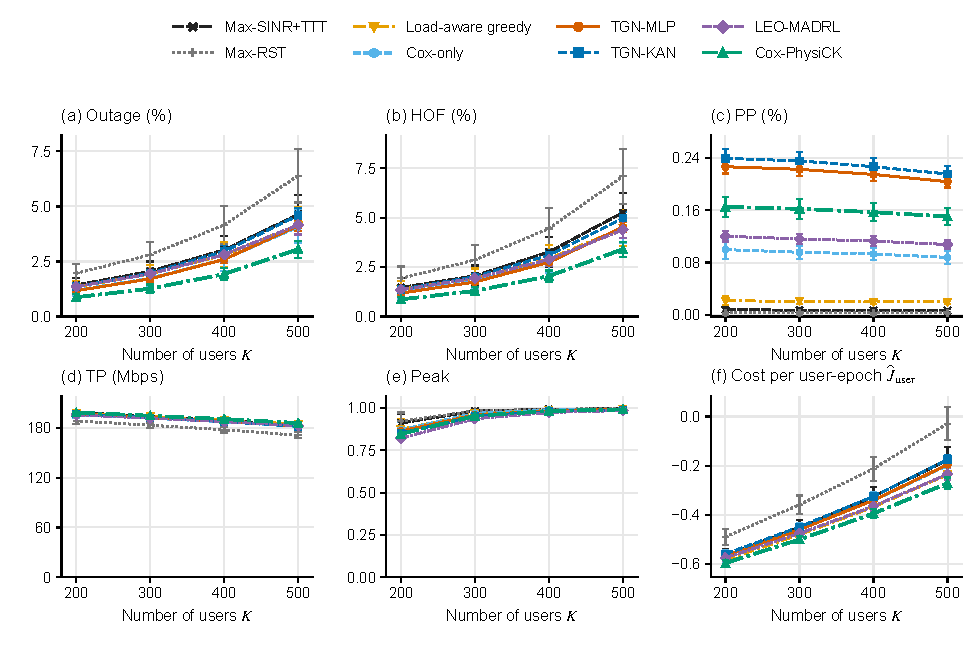
\includegraphics[width=\textwidth]{figures/figure_3.pdf}
\caption{\revnew{User-density shift at $N_{\rm sat}=2000$ and $H=200$. Learned controllers are trained at $K=100$ and evaluated without retraining at $K=200$--$500$; the nominal results appear in Table~\ref{tab:traditional_baselines}. Panels show (a) outage, (b) conditional HO failure, (c) PP, (d) TP, (e) Peak, and (f) cost per user--epoch. Error bars denote sample SD across five seed means for learned methods and across valid episodes for deterministic methods.}}
\label{fig:ood_generalization}
\end{figure*}



\revnew{Figure~\ref{fig:ood_generalization} tests all eight methods at $K=200$--$500$, with learned parameters, normalizers, and KAN grids frozen after $K=100$ training. HOF rises with density for every method, but Cox-PhysiCK retains the lowest observed mean. Its absolute HOF gap from greedy widens, although the relative reduction falls from $34.8\%$ at $K=100$ to $23.8\%$ at $K=500$. At the latter density, TP is highest for Cox-PhysiCK, while its PP remains higher than greedy and LEO-MADRL. Peak approaches one for all methods and offers little discrimination; served-only P5TP is also similar, near 58\,Mbps.}

\revnew{At $K=500$, the mean cost difference from greedy is $-0.0356$, with a conditional 95\% interval of $[-0.0646,-0.0065]$. The observed difference from LEO-MADRL is $-0.0368$. The advantage over greedy mainly comes from the outage term at $w_o=5$. The weighted outage, switching, load, and negative-rate differences are respectively $-0.01615$, $+0.00613$, $+0.00308$, and $-0.00289$ at $K=100$, and $-0.05480$, $+0.00586$, $+0.01942$, and $-0.00603$ at $K=500$. Thus greedy incurs lower average switching and load penalties, despite its higher total cost. Peak cannot replace the average load term.}

\subsection{\revnew{Calibration and Parameter Sensitivity}}
\label{subsec:calibration_sensitivity}

\subsubsection{\revnew{Calibration factor}}
\revnew{Figure~\ref{fig:kappa-sensitivity} tests the zero-arrival descriptor under prescribed frozen retention at 535--565\,km, using each trace's geometry for exposure. Independent geometric-entry calibration gives $\hat\kappa=0.6033$ with a 95\% trace-bootstrap interval of $[0.5832,0.6235]$. Held-out diagnostics scan $\kappa=0.30,0.45,0.60,0.75,0.90$ to assess the controller's preset $\kappa_0=0.60$.}

\revnew{Panel (a) gives predicted and empirical void rates, macro-averaged over six window lengths: $0.4136$ and $0.4158$ at $\kappa_0$. All settings use the same windows and labels. Panel (b)'s lowest mean Brier score is $0.1586$ at $\kappa=0.60$, but the shallow minimum weakly distinguishes nearby settings. This diagnostic tests arrival predictions under prescribed thinning. It does not test the frozen-retention assumption or establish calibration at every window length.}

\begin{figure*}[t]
\centering
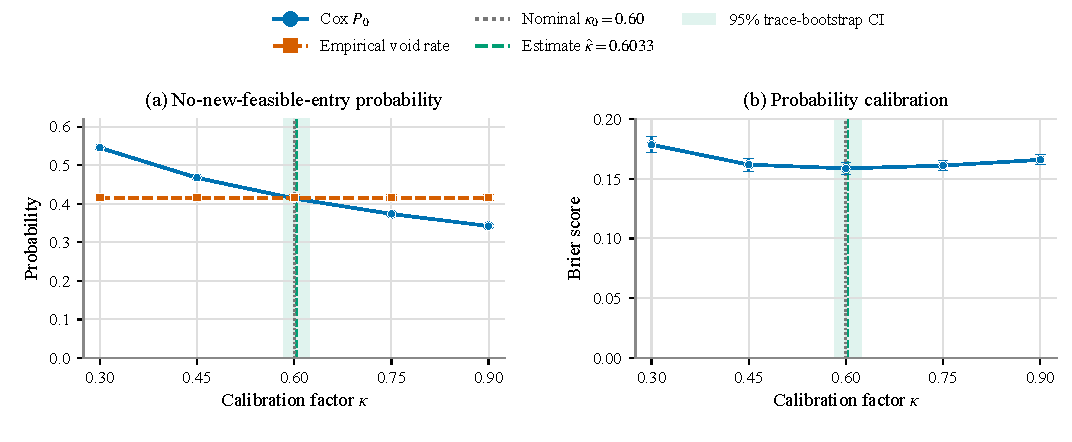
\includegraphics[width=\textwidth]{figures/figure_4.pdf}
\caption{\revnew{Cox diagnostic with independent frozen-retention thinning: (a) void probabilities; (b) Brier score. Points/bars show means/sample SD of five seed macro-means over six window lengths.}}
\label{fig:kappa-sensitivity}
\end{figure*}


\subsubsection{\revnew{Cost weights}}
\revnew{Figure~\ref{fig:weight-sensitivity} varies one coordinate of $(5,0.5,0.5,1)$ at a time, with separately trained models for all 17 unique configurations. At $1.5\times$ the nominal weight, the mean PP ratio is $0.677$ for $w_h$ and the mean Peak ratio is $0.963$ for $w_\ell$.  Mean outage and HOF changes are nonmonotonic and accompanied by broad seed dispersion; this does not establish insensitivity, since some mean changes approach $30\%$. TP changes remain within approximately $-1.1\%$ to $+0.8\%$ over the scan. No configuration improves all five mean metrics.}

\begin{figure*}[!t]
    \centering
    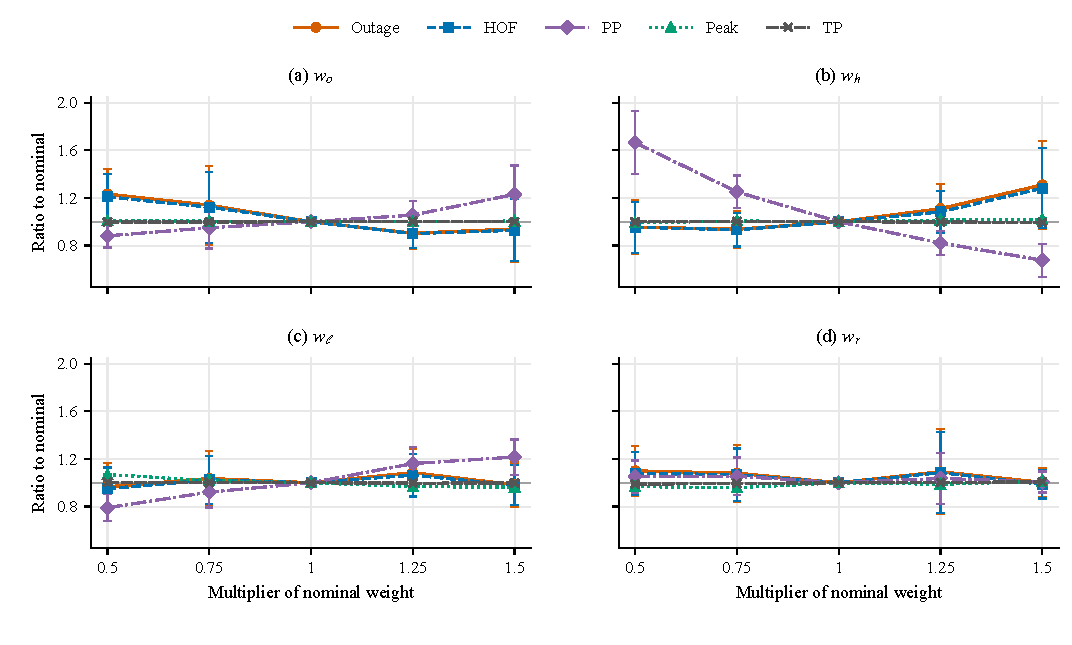
\includegraphics[width=\textwidth]{figures/figure_5.pdf}
    \caption{\revnew{Cost-weight sensitivity at $N_{\rm sat}=2000$, $K=100$, $H=200$. Each panel varies one nominal weight with separate training. Points/bars: mean/sample SD of five seed-indexed ratios after episode averaging. Nominal ratios equal one. Higher TP and lower other metrics are preferable.}}
\label{fig:weight-sensitivity}
\end{figure*}

\subsubsection{\revnew{Decision hysteresis}}
\revnew{Table~\ref{tab:hysteresis_sensitivity} varies test-time hysteresis at fixed models and episodes; $w_h C_k^{\rm exec}$ separately penalizes switching. For Cox-PhysiCK, raising $\tau_{\rm hyst}$ from $0.05$ to $0.30$ reduces PP from $0.165\%$ to $0.035\%$, while outage rises from $0.609\%$ to $0.674\%$, conditional HO failure from $0.618\%$ to $0.692\%$, and executed HO frequency falls from $5.51$ to $3.02$ per user-minute. Cox-only shows the same switching--reliability direction. Greedy\textquotesingle s PP falls by about $80\%$. At matched margins, Cox-PhysiCK retains seven to eight times greedy\textquotesingle s PP; hysteresis alone does not explain this gap. The nominal comparison retains the preset $0.05$ margin.}

\begin{table*}[t]
\centering
\caption{Test-time hysteresis sensitivity at $N_{\rm sat}=2000$, $K=100$, and $H=200$.}
\label{tab:hysteresis_sensitivity}
\footnotesize
\renewcommand{\arraystretch}{1.1}
\setlength{\tabcolsep}{3pt}
\begin{tabularx}{\textwidth}{@{}l c *{4}{>{\centering\arraybackslash}X} c@{}}
\toprule
Method & $\tau_{\rm hyst}$ & Out. (\%) & Fail (\%) & PP (\%) & TP (Mbps) & $\widehat J_{\rm user}$ \\
\midrule
Load-aware greedy & 0.10 & \revnew{$0.953\pm0.204$} & \revnew{$0.959\pm0.465$} & \revnew{$0.016\pm0.007$} & \revnew{$201.89\pm3.74$} & \revnew{$-0.6796\pm0.0228$} \\
 & 0.20 & \revnew{$0.992\pm0.216$} & \revnew{$1.033\pm0.531$} & \revnew{$0.009\pm0.006$} & \revnew{$201.79\pm3.79$} & \revnew{$-0.6780\pm0.0239$} \\
 & 0.30 & \revnew{$1.032\pm0.225$} & \revnew{$1.025\pm0.588$} & \revnew{$0.005\pm0.005$} & \revnew{$201.70\pm3.81$} & \revnew{$-0.6764\pm0.0241$} \\
\midrule
Cox-only & 0.10 & \revnew{$0.850\pm0.186$} & \revnew{$0.880\pm0.315$} & \revnew{$0.073\pm0.015$} & \revnew{$200.40\pm3.73$} & \revnew{$-0.6679\pm0.0223$} \\
 & 0.20 & \revnew{$0.887\pm0.191$} & \revnew{$0.927\pm0.383$} & \revnew{$0.039\pm0.012$} & \revnew{$200.36\pm3.70$} & \revnew{$-0.6684\pm0.0215$} \\
 & 0.30 & \revnew{$0.920\pm0.197$} & \revnew{$0.943\pm0.450$} & \revnew{$0.021\pm0.010$} & \revnew{$200.29\pm3.71$} & \revnew{$-0.6678\pm0.0222$} \\
\midrule
\textbf{Cox-PhysiCK} & 0.10 & \revnew{$0.620\pm0.091$} & \revnew{$0.625\pm0.084$} & \revnew{$0.120\pm0.013$} & \revnew{$202.57\pm0.96$} & \revnew{$-0.6899\pm0.0089$} \\
 & 0.20 & \revnew{$0.646\pm0.094$} & \revnew{$0.655\pm0.090$} & \revnew{$0.066\pm0.007$} & \revnew{$202.49\pm0.98$} & \revnew{$-0.6900\pm0.0092$} \\
 & 0.30 & \revnew{$0.674\pm0.099$} & \revnew{$0.692\pm0.103$} & \revnew{$0.035\pm0.003$} & \revnew{$202.46\pm0.98$} & \revnew{$-0.6907\pm0.0092$} \\
\bottomrule
\end{tabularx}
\par\vspace{3pt}
\begin{minipage}{\textwidth}\footnotesize
\revnew{The nominal $\tau_{\rm hyst}=0.05$ results are in Table~\ref{tab:traditional_baselines}.}
\end{minipage}
\end{table*}


\Needspace{10\baselineskip}
\noindent\begin{minipage}{\columnwidth}
\section{Conclusion}
\label{sec:conclusion}
\revnew{Cox-PhysiCK combines calibrated Cox arrival descriptors with physics-conditioned temporal messages for coupled handover control. In the SGP4-propagated synthetic Walker scenarios, it reduces mean outage and conditional HO failure relative to the TGN baselines at the reported horizons. Its observed gaps from greedy in outage, conditional HO failure, and cost widen at 500 users; the cost gain is driven mainly by outage under $w_o=5$, with higher switching and load penalties. Cox and ephemeris descriptors show mixed performance differences. The analysis provides local perturbation bounds under fixed decision sets. Results concern stationary terminals. Deployment requires updating $\kappa$ from observed entry statistics and aligning SINR/load measurements, admission, and execution with 3GPP reporting and handover timelines; mobile users and multi-layer operation remain future work.}


\end{minipage}
\appendices

\section{\textcolor{blue}{Derivation of the Cox Zero-Arrival Probability}}
\label{app:cox_risk}

\textcolor{blue}{Over $(t,t+T]$, $0<T<2\pi/\theta$, the locally frozen-plane approximation retains one count $M_k(t)\sim\operatorname{Poisson}(\rho)$ throughout. The prescribed profile $\bar p_k(u;t)\in[0,1]$ independently thins entries with equal probability across planes and is fixed when averaging over the prior; it does not reveal future realized SINR or load.}

\textcolor{blue}{During $du$, the swept phase interval has length $\theta\,du$, giving the phase-PPP ideal rate $Q\theta/(2\pi)$; scaling by $\kappa$ gives $\beta=\kappa Q\theta/(2\pi)$. The retained entry count per plane has mean}
\[
\textcolor{blue}{A_k(t,T)=\beta\int_t^{t+T}\bar p_k(u;t)\,du.}
\]
\textcolor{blue}{Conditioned on $M_k(t)=m$, independent thinning and superposition give}
\[
\textcolor{blue}{
N_k^{\rm feas}(t,T)\mid M_k(t)=m
\sim\operatorname{Poisson}\!\left(mA_k(t,T)\right).
}
\label{eq:poisson_count_app}
\]
\textcolor{blue}{The conditional void probability is}
\[
\textcolor{blue}{
\Pr\!\left\{N_k^{\rm feas}(t,T)=0\mid M_k(t)=m\right\}
=e^{-mA_k(t,T)}.
}
\label{eq:void_cont_app}
\]
\textcolor{blue}{Averaging over the Poisson plane count yields}
\[
\textcolor{blue}{
\begin{aligned}
\Pr\!\left\{N_k^{\rm feas}(t,T)=0\right\}
&=\sum_{m=0}^{\infty}e^{-mA_k(t,T)}\frac{e^{-\rho}\rho^m}{m!}\\
&=\exp\!\left[-\rho\left(1-e^{-A_k(t,T)}\right)\right].
\end{aligned}
}
\label{eq:cox_risk_cont_app}
\]
\textcolor{blue}{Replacing $M_k(t)$ by its mean $\rho$ before averaging instead gives $e^{-\rho A_k(t,T)}$, the mean-intensity Poisson approximation. The Cox expression retains plane-count randomness.}

\textcolor{blue}{For a piecewise-constant profile $\bar p_{k,j|t}$, let $J(T)=\lceil T/\Delta t\rceil$ and $\delta_j(T)=\min\{\Delta t,T-j\Delta t\}$.
Its per-plane mean entry count is}
\[
\textcolor{blue}{A_k^\Delta(t,T)=\beta\sum_{j=0}^{J(T)-1}\bar p_{k,j|t}\delta_j(T).}
\]
\textcolor{blue}{For the common user window $T$ specified in Section~\ref{subsec:cox_main}, the resulting descriptor is}
\[
\textcolor{blue}{
P_{0,k}(t)
=\exp\!\left[-\rho\left(1-e^{-A_k^\Delta(t,T)}\right)\right],
}
\label{eq:cox_risk_discrete_app}
\]
\textcolor{blue}{recovering \eqref{eq:Prisk_def_main}. For the grid-based RST in \eqref{eq:geometry_rst}, all interval weights equal $\Delta t$.}

\textcolor{blue}{
The sum exactly integrates the prescribed piecewise-constant profile. Approximating future feasibility by this profile introduces mismatch when load or beam activation changes. Lemma~\ref{lem:cox_risk_calibration} bounds the descriptor error through integrated mean-rate error.
}
\revnew{Freeze-decide-update fixes current information, not future feasibility; reducing $\Delta t$ or refreshing descriptors cannot alone eliminate full-window mismatch from frozen retention.}



\section{\revnew{Numerical Implementation}}
\label{app:implementation}
\begingroup
\color{red}

\begin{table}[!t]
\color{red}\centering\footnotesize
\caption{Message and coefficient modules. Shared memories and readouts are excluded.}
\label{tab:message_implementations}
\setlength{\tabcolsep}{3pt}
\begin{tabular}{@{}lcr@{}}
\toprule
Module & Mapping & Parameters \\
\midrule
TGN-MLP / no-kernel & $262\to213\to128$ & 83,411 \\
TGN-KAN message & $262\to32\to128$ & 112,480 \\
KAN coefficient head & $262\to32\to10$ & 78,378 \\
Full message, including bank & --- & 83,498 \\
MLP coefficient head & $262\to287\to10$ & 78,361 \\
\bottomrule
\end{tabular}
\end{table}

\subsection{Geometry and Message Implementation}
Users are sampled uniformly in longitude and sine latitude within Table~\ref{tab:sim_params}'s region and remain stationary per episode. The Walker constellation uses equally spaced planes with phasing $F=1$. Shared beam schedules and weather traces are exogenous. Subbands are orthogonal within satellites and fully reused across satellites. The elevation-equivalent visibility test uses $d_{\rm norm}=2d/d_{\max}\le2$, with
\[
d_{\max}=\sqrt{(R_e+h)^2-R_e^2\cos^2e_{\min}}-R_e\sin e_{\min}.
\]
Propagation extends beyond each episode to determine geometric RST.

For either antenna, the gain in dBi at off-axis angle $\psi$ is
\[
G_{\rm dBi}(\psi)=G_{\max,\rm dBi}
-\min\!\left\{12(\psi/\theta_{3\rm dB})^2,A_{\max}\right\},
\]
using the full 3\,dB beamwidth $\theta_{3\rm dB}$ and attenuation cap $A_{\max}$ in Table~\ref{tab:sim_params}. Gains are converted to linear units for the link equations.
Gas loss is always 0.12\,dB. The rain state has probability 0.10 and remains fixed per episode, adding 5\,dB on affected links. Blockage adds 8\,dB, with per-second transition probabilities 0.1 from blocked to clear and 0.005263 from clear to blocked, giving approximately 5\% stationary blockage and 10\,s mean duration.

The physical coordinates are
\[
\mathbf u=\operatorname{clip}_{[0,1]}\!\left(
P_{0,k},\frac{\log(1+\Lambda_k^{\rm n})}{\log11},
\frac{\log(1+T_{\nu,k}^{\rm n})}{\log21}\right).
\]
With $\psi_0(u)=1-u$ and $\psi_1(u)=u$, the eight products $\psi_r(u_1)\psi_q(u_2)\psi_v(u_3)$, $r,q,v\in\{0,1\}$, together with $\kappa_{\rm surv}$ and $\kappa_{\rm load}$ form the ten-kernel bank. Basis shapes are fixed; $\mathbf W_m$ and the coefficient head are learned. The KAN uses fixed grids on $[-1,1]$, boundary-saturated cubic splines, a SiLU base branch, and temperature-one softmax. Each connection has eight spline coefficients and one base coefficient, plus output-node biases. Physical kernels retain physical units before the stated normalization; learned inputs use training-set standardization, frozen for evaluation.





\subsection{Training and Descriptor Interventions}
\label{app:training_implementation}
Residual training uses four rounds, each with 80 episodes and 5,000 AdamW updates, collecting data with the analytic policy first and the preceding learned policy thereafter. Uniform feasible-candidate exploration is 0.20, 0.15, 0.10, and 0.05 by round. After 500 warmup updates, learning rate decays from $3\times10^{-4}$ to $3\times10^{-5}$; weight decay is $10^{-5}$. Batches contain four 64-step sequences, with 32 burn-in steps followed by 32 loss-bearing steps. The nonempty-request target $q^{\rm target}_{k,b}=-c_k-U^{\rm ana}_{k,b}$ uses the final outcome, including rejection or fallback. The loss is
\[
\mathcal L=\operatorname{MSE}_{\mathcal B_{\rm req}}(\widehat Q,q^{\rm target})
+0.1\operatorname{MSE}_{\mathcal B_{\rm edge}}
(\widehat y,\ell_\nu/\ell_\nu^{\max}).
\]
MSE averages nonempty requested edges in $\mathcal B_{\rm req}$ and valid preselected edges in $\mathcal B_{\rm edge}$; the latter targets each edge's satellite occupancy after execution. Padding and empty terms are omitted. The auxiliary head is excluded from control; the residual final layer starts at zero.

The no-arrival/RST variant masks all three physical descriptors throughout the bank and learned inputs. The no-Cox, RST-retained variant masks only $P_0$ and the entry rate and replaces the candidate zero-arrival kernel by one. Ephemeris-PhysiCK substitutes
\[
\begin{aligned}
P^{\rm eph}_0(t,T)&=(1-p)^{n^{\rm ent}(t,T)},\\
\Lambda^{\rm eph}(t,T)&=p\,n^{\rm ent}(t,T)/T.
\end{aligned}
\]
where $p=p_{{\rm feas},k}(t)$ is frozen and $n^{\rm ent}$ counts geometric satellite entries on the one-second grid. Currently visible satellites are excluded. At $T=0$, probability is one and rate zero. Common-window features and candidate-RST kernels use their respective original windows, with no $\kappa$ applied to known entries. Each variant is retrained.

\subsection{Analytical Comparators}
\label{app:cox_only_spec}
Using greedy's analytic utility from \eqref{eq:analytic_utility}, Cox-only scores candidates by
\[
S^{\rm Cox}_{k,\nu,n}=U^{\rm ana}_{k,\nu,n}-P^{\rm cand}_{0,k,\nu},
\]
\[
P^{\rm cand}_{0,k,\nu}=\exp\!\left[-\rho\left(1-e^{-A_k^\Delta(t,T^{\rm rst}_{\nu,k})}\right)\right].
\]
The candidate-specific RST prevents cancellation of the penalty in score differences; the main controller's common-window descriptor is unchanged.

\subsection{LEO-MADRL}
\label{app:adapted_dqn}
LEO-MADRL adapts the hysteretic-learning principle of~\cite{10551688}, rather than reproducing its complete successive algorithm. It uses our observations, masked actions, reward, and joint execution, sharing $73\to128\to128\to9$ ReLU online/target networks and replay across users. Its eight slots contain
\[
\begin{gathered}
P_0,\quad\log(1+\Lambda^{\rm feas}T_{\rm ref}),\quad
\log(1+T^{\rm rst}/T_{\rm ref}),\\
\tilde\gamma,\quad\tilde\ell/10,\quad C,\\
\mathbf1\{b=s_k\},\ \mathbf1\{\text{slot exists}\},\
\mathbf1\{b\in\tilde{\mathcal A}_k\},
\end{gathered}
\]
plus an empty-source indicator. Slots use decreasing frozen SINR, then IDs. Continuous features are standardized; missing/infeasible actions are masked throughout. The ninth action requires an empty feasible set. Requests precede joint execution, followed by one shared minibatch update per epoch after collecting 10,000 user transitions. No additional utility hysteresis or TTT applies. Reward is $-c_k$, discount $0.99$, and the TD target uses the direct target-network maximum. Detached weights of 1 for nonnegative TD error and $0.2$ otherwise multiply Huber$_1$ loss. Adam uses learning rate $10^{-4}$, batch 128, and replay 100,000. Every 1,000 optimizer updates, targets synchronize and checkpoints are evaluated; selection minimizes validation cost among positive checkpoints. Exploration decays linearly from 1 to 0.05 over the first 102,400 of 256,000 epochs, then remains fixed; evaluation disables exploration.

\subsection{Calibration}
Calibration and held-out diagnostics use $5\times30$ and $5\times60$ 800\,s traces, respectively, each with 2000 satellites and ten users. The estimator $\widehat\kappa=\sum_j C_j/\sum_j E_j$ uses unfiltered entries and exposure at $\kappa=1$. Ten thousand bootstrap replicates resample complete traces within seeds. The preset $\kappa=0.60$ is fixed before testing. Each user's six windows (10, 30, 60, 120, 240, 480\,s) share a uniformly sampled integer start in $[0,320]$\,s. Diagnostic retention $p_{\rm diag}=F_{\rm diag}/V_{\rm diag}$ uses prescribed count pairs, with zero for an empty denominator. The 3,000 trace--user count pairs and window mappings are supplied in the accompanying data archive. Their ratios span $[0,1]$ (mean $0.503$), remain fixed across six windows, and differ from \eqref{eq:p_feas}. Independent uniform marks retain entries with probability $p_{\rm diag}$; no retained entry in $(t,t+T]$ defines a void. These 18,000 windows assess prescribed thinning without controller-generated loads. Plots report mean and sample SD of five seed summaries, equally weighting window lengths.

\endgroup


\bibliographystyle{IEEEtran}
\bibliography{references}



 \vfill

\end{document}
